\documentclass[11pt,]{book}
\usepackage{lmodern}
\usepackage{setspace}
\setstretch{2}
\usepackage{amssymb,amsmath}
\usepackage{ifxetex,ifluatex}
\usepackage{fixltx2e} % provides \textsubscript
\ifnum 0\ifxetex 1\fi\ifluatex 1\fi=0 % if pdftex
  \usepackage[T1]{fontenc}
  \usepackage[utf8]{inputenc}
\else % if luatex or xelatex
  \ifxetex
    \usepackage{mathspec}
  \else
    \usepackage{fontspec}
  \fi
  \defaultfontfeatures{Ligatures=TeX,Scale=MatchLowercase}
\fi
% use upquote if available, for straight quotes in verbatim environments
\IfFileExists{upquote.sty}{\usepackage{upquote}}{}
% use microtype if available
\IfFileExists{microtype.sty}{%
\usepackage{microtype}
\UseMicrotypeSet[protrusion]{basicmath} % disable protrusion for tt fonts
}{}
\usepackage[margin=1in]{geometry}
\usepackage{hyperref}
\hypersetup{unicode=true,
            pdfborder={0 0 0},
            breaklinks=true}
\urlstyle{same}  % don't use monospace font for urls
\usepackage{natbib}
\bibliographystyle{apalike}
\usepackage{color}
\usepackage{fancyvrb}
\newcommand{\VerbBar}{|}
\newcommand{\VERB}{\Verb[commandchars=\\\{\}]}
\DefineVerbatimEnvironment{Highlighting}{Verbatim}{commandchars=\\\{\}}
% Add ',fontsize=\small' for more characters per line
\usepackage{framed}
\definecolor{shadecolor}{RGB}{248,248,248}
\newenvironment{Shaded}{\begin{snugshade}}{\end{snugshade}}
\newcommand{\KeywordTok}[1]{\textcolor[rgb]{0.13,0.29,0.53}{\textbf{{#1}}}}
\newcommand{\DataTypeTok}[1]{\textcolor[rgb]{0.13,0.29,0.53}{{#1}}}
\newcommand{\DecValTok}[1]{\textcolor[rgb]{0.00,0.00,0.81}{{#1}}}
\newcommand{\BaseNTok}[1]{\textcolor[rgb]{0.00,0.00,0.81}{{#1}}}
\newcommand{\FloatTok}[1]{\textcolor[rgb]{0.00,0.00,0.81}{{#1}}}
\newcommand{\ConstantTok}[1]{\textcolor[rgb]{0.00,0.00,0.00}{{#1}}}
\newcommand{\CharTok}[1]{\textcolor[rgb]{0.31,0.60,0.02}{{#1}}}
\newcommand{\SpecialCharTok}[1]{\textcolor[rgb]{0.00,0.00,0.00}{{#1}}}
\newcommand{\StringTok}[1]{\textcolor[rgb]{0.31,0.60,0.02}{{#1}}}
\newcommand{\VerbatimStringTok}[1]{\textcolor[rgb]{0.31,0.60,0.02}{{#1}}}
\newcommand{\SpecialStringTok}[1]{\textcolor[rgb]{0.31,0.60,0.02}{{#1}}}
\newcommand{\ImportTok}[1]{{#1}}
\newcommand{\CommentTok}[1]{\textcolor[rgb]{0.56,0.35,0.01}{\textit{{#1}}}}
\newcommand{\DocumentationTok}[1]{\textcolor[rgb]{0.56,0.35,0.01}{\textbf{\textit{{#1}}}}}
\newcommand{\AnnotationTok}[1]{\textcolor[rgb]{0.56,0.35,0.01}{\textbf{\textit{{#1}}}}}
\newcommand{\CommentVarTok}[1]{\textcolor[rgb]{0.56,0.35,0.01}{\textbf{\textit{{#1}}}}}
\newcommand{\OtherTok}[1]{\textcolor[rgb]{0.56,0.35,0.01}{{#1}}}
\newcommand{\FunctionTok}[1]{\textcolor[rgb]{0.00,0.00,0.00}{{#1}}}
\newcommand{\VariableTok}[1]{\textcolor[rgb]{0.00,0.00,0.00}{{#1}}}
\newcommand{\ControlFlowTok}[1]{\textcolor[rgb]{0.13,0.29,0.53}{\textbf{{#1}}}}
\newcommand{\OperatorTok}[1]{\textcolor[rgb]{0.81,0.36,0.00}{\textbf{{#1}}}}
\newcommand{\BuiltInTok}[1]{{#1}}
\newcommand{\ExtensionTok}[1]{{#1}}
\newcommand{\PreprocessorTok}[1]{\textcolor[rgb]{0.56,0.35,0.01}{\textit{{#1}}}}
\newcommand{\AttributeTok}[1]{\textcolor[rgb]{0.77,0.63,0.00}{{#1}}}
\newcommand{\RegionMarkerTok}[1]{{#1}}
\newcommand{\InformationTok}[1]{\textcolor[rgb]{0.56,0.35,0.01}{\textbf{\textit{{#1}}}}}
\newcommand{\WarningTok}[1]{\textcolor[rgb]{0.56,0.35,0.01}{\textbf{\textit{{#1}}}}}
\newcommand{\AlertTok}[1]{\textcolor[rgb]{0.94,0.16,0.16}{{#1}}}
\newcommand{\ErrorTok}[1]{\textcolor[rgb]{0.64,0.00,0.00}{\textbf{{#1}}}}
\newcommand{\NormalTok}[1]{{#1}}
\usepackage{longtable,booktabs}
\usepackage{graphicx,grffile}
\makeatletter
\def\maxwidth{\ifdim\Gin@nat@width>\linewidth\linewidth\else\Gin@nat@width\fi}
\def\maxheight{\ifdim\Gin@nat@height>\textheight\textheight\else\Gin@nat@height\fi}
\makeatother
% Scale images if necessary, so that they will not overflow the page
% margins by default, and it is still possible to overwrite the defaults
% using explicit options in \includegraphics[width, height, ...]{}
\setkeys{Gin}{width=\maxwidth,height=\maxheight,keepaspectratio}
\IfFileExists{parskip.sty}{%
\usepackage{parskip}
}{% else
\setlength{\parindent}{0pt}
\setlength{\parskip}{6pt plus 2pt minus 1pt}
}
\setlength{\emergencystretch}{3em}  % prevent overfull lines
\providecommand{\tightlist}{%
  \setlength{\itemsep}{0pt}\setlength{\parskip}{0pt}}
\setcounter{secnumdepth}{5}
% Redefines (sub)paragraphs to behave more like sections
\ifx\paragraph\undefined\else
\let\oldparagraph\paragraph
\renewcommand{\paragraph}[1]{\oldparagraph{#1}\mbox{}}
\fi
\ifx\subparagraph\undefined\else
\let\oldsubparagraph\subparagraph
\renewcommand{\subparagraph}[1]{\oldsubparagraph{#1}\mbox{}}
\fi

%%% Use protect on footnotes to avoid problems with footnotes in titles
\let\rmarkdownfootnote\footnote%
\def\footnote{\protect\rmarkdownfootnote}

%%% Change title format to be more compact
\usepackage{titling}

% Create subtitle command for use in maketitle
\newcommand{\subtitle}[1]{
  \posttitle{
    \begin{center}\large#1\end{center}
    }
}

\setlength{\droptitle}{-2em}
  \title{}
  \pretitle{\vspace{\droptitle}}
  \posttitle{}
  \author{}
  \preauthor{}\postauthor{}
  \date{}
  \predate{}\postdate{}

\usepackage{booktabs}
\usepackage{amsthm}
\usepackage[utf8]{inputenc}
\usepackage[english]{babel}
\makeatletter
\def\thm@space@setup{%
  \thm@preskip=8pt plus 2pt minus 4pt
  \thm@postskip=\thm@preskip
}
\makeatother
\pagenumbering{roman}

\usepackage{amsthm}
\newtheorem{theorem}{Theorem}[chapter]
\newtheorem{lemma}{Lemma}[chapter]
\theoremstyle{definition}
\newtheorem{definition}{Definition}[chapter]
\newtheorem{corollary}{Corollary}[chapter]
\newtheorem{proposition}{Proposition}[chapter]
\theoremstyle{definition}
\newtheorem{example}{Example}[chapter]
\theoremstyle{remark}
\newtheorem*{remark}{Remark}
\begin{document}

\begin{center}
\bf{The Pennsylvania State University} \\
The Graduate School \\
College of Medicine Public Health Sciences \\


STATISITCAL MODELS FOR HIGH DIMENSIONAL SCREENING OF GENETIC AND EPIGENETIC EFFECTS
(maybe include something about GWAS and functional values?)

A Dissertation in \\
Biostatistics \\
by \\
Kirk Gosik \\
(c) 2017 Kirk Gosik \\

Doctor of Philosophy \\
February 2017 \\

\newpage

The dissertation of Kirk Gosik was reviewed and approved* by the following:

Rongling Wu \\
Distinguished Professor of Public Health Sciences and Statistics \\
Thesis Advisor, Chair of Committee

Vernon Chinchilli \\
Distinguished Professor and Chair of Public Health Sciences


Lan Kong \\
Associate Professor of Public Health Sciences

James Broach \\
Distinguished Professor and Chair of Biochemistry and Molecular Biology \\


\newpage

Abstract

Knowledge about how changes in gene expression are encoded by expression quantitative trait loci (eQTLs) is a key to construct the genotype-phenotype map for complex traits or diseases. Traditional eQTL mapping is to associate one transcript with a single marker at a time, thereby limiting our inference about a complete picture of the genetic architecture of gene expression. Here, I present innovative applications of variable selection approaches to systematically detect main effects and interaction effects among all possible loci on differentiation and function of gene expression and other phenotypes of interest. Forward-selection-based procedures were particularly implemented to tackle complex covariance structures of gene-gene interactions. Simulation studies were performed on each of the models to assess the computational properties of each model.  Applications of the models were also performed on real datasets.  The first was a reanalysis of a published genetic and genomic dataset collected in a mapping population of Caenorhabditis elegans, gaining new discoveries on the genetic origin of gene expression differentiation, which could not be detected by a traditional one-locus/one-transcript analysis approach.  The next dataset was of Mei Tree growth, analyzing the genetic control of the height and diameter during the developmental process.  The underlying genotypes and epistasis that impact the process of these developments were considered as candidates for the selection of the procedure.

\end{center}

{
\setcounter{tocdepth}{1}
\tableofcontents
}
\listoftables
\listoffigures
\chapter{Introduction}\label{intro}

\pagenumbering{arabic} \setcounter{page}{1}

\section{Background}\label{background}

There are several techniques used for studying genetics and mapping the
results. Some of the more populor techniques include cross-breeding
experiments or, in the case of humans, the examination of family
histories, known as pedigrees. More recently, CRISPR/Cas9 can be used to
mimic mitotic recombination to help map out genes as well.
(\cite{sadhu2016crispr})

Construction of genetic maps are a variety of techniques used to show
relative positions between genes or other sequence features of the
genome and the phenotype that is controlled by such sequences. Genes are
very useful markers but they are by no means ideal. One problem,
especially with larger genomes such as those of vertebrates and
flowering plants, is that a map based entirely on genes is not very
detailed.(\cite{brown2006genomes}) Genes have long areas of non-coding
regions between them and therefore result in large gaps from gene to
gene. This is further complicated because not every gene has allelic
forms that can be easily or conventiently distinguished. With these
considerations in mind gene maps may not be comprehensive enough and
other markers may be needed.

According to brown, mapped features that are not genes are called DNA
markers. As with gene markers, a DNA marker must have at least two
alleles to be useful. There are three types of DNA sequence feature that
satisfy this requirement: restriction fragment length polymorphisms
(RFLPs), simple sequence length polymorphisms (SSLPs), and single
nucleotide polymorphisms (SNPs). (\cite{brown2006genomes}) The genetic
markers that have been emphaised in this work are single nucleotide
polymorphisms. Attempting to be at the highest levels of resolution for
identifying quantitative traits, using SNPs are the most specific case.
This will give exact location of the nucletid that may be impacting the
genetic control over the phenotype.

\begin{figure}

{\centering 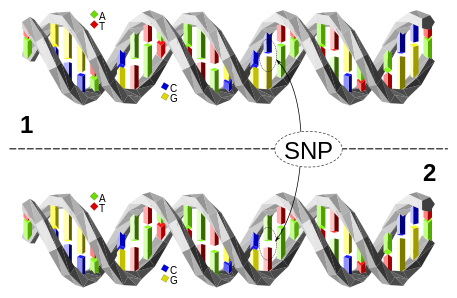
\includegraphics[width=0.8\linewidth]{images/SNP_Picture} 

}

\caption{SNP Picture}\label{fig:Snp-Pic}
\end{figure}

There are several goals to genetic mapping and association studies that
identify certain regions of the genome that contain genes involved in
specifying a quantitative trait, refered to as quantitative trait loci
(QTLs). One main goal is to estimate the genetic effects of these loci.
The relationship between the genetic effects of QTLs and the phenotypic
value of quantitative traits can be described by a linear model
(\cite{collard2005introduction}, \cite{xu2007empirical}). Typically,
because of the high throughput nature of the data there are a large
number of markers across the whole genome, and most of the markers may
have very little or next no effect on the phenotype under study. The
models can be very sparse, with most cases, the number of genetic
markers or variables is bigger than the sample size, especially when
interactions among markers are considered. This makes a model is
oversaturated and furher model selection techniques may be required to
capture the necessary information. \cite{dong2015accurate}

\section{Some Exisiting Methods}\label{some-exisiting-methods}

Numerous methods exist and are being developed to measure and find
quantitative trait loci (QTL) effects. These methods can broadly fall
into three main categories. These categories are Least-Square methods,
maximum likelihood and Bayesian approaches. (\cite{wu2007statistical})
Each method has advantages and considerations that you would need to be
aware before conducting analyses to find QTL effects from the given
markers. A brief discussions on a few of the methods are given to
highlight some areas of consideration and how the methods proposed can
handle such considerations.

Marker Regression would fall in the category of Least Squares
approaches. If looking at one marker analysis general t-test and ANOVA
procedures can be used to analyze the relationship. It is not
recommended however for use in general practice because you do not know
how dense the markers are measured. QTL interval mapping would be
preferred in such an analysis because the methods take account for
missing genotype data that may not have been measured. When estimating a
QTL position through maximum likelihood methods, like interval mapping,
positions of other possible QTLs could affect the detection of the true
position. Neighboring QTLs could possibly flatten the likelihood in
instances where there are multiple QTLs on the same chromosome. This
would make an effect look less significant at a given location than it
actually is. Another possibility is that in the search over the interval
you may find an area where the likelihood could reach a peak but could
be a ``ghost'' QTL. This is where an effect is observed because a
neighboring QTL is skewing the results at the particular position you
are looking in and the result is a false discovery of the position.
Marker Regression has been shown to improve interval mapping, which is
call Composite Interval Mapping. This is where the QTL position found is
also combined in a linear regression where the covariates are the other
markers in the dataset. By including the markers as covariates the other
position in the chromosome are accounted for in the analysis and false
discovery is reduced.

The analysis of interval mapping and single marker analyses has shown to
be effective but it limits our inference to one marker at a time as a
possible loci that controls a trait. Using Marker Regression however you
can incorporate multiple markers in a single analysis to test for
possible QTL for a given trait. It is cautioned that running such an
analysis is only an approximate test because the null hypothesis is
there is no difference between the marker levels and therefore a
non-mixture distribution but the alternative is a mixture of
distributions. The assumptions regression would make of the errors
within the marker type to be normally distributed may not be entirely
met if the QTL's fall between the marker regions. However
\cite{whittaker1996mapping} have shown that a direct regression of
phenotypes on marker types, provides the same information about location
of QTL-effects without having to step to all positions on the interval.
With this information using the entire marker set in a regression
analysis would provide a nice, computationally efficient way to map out
the genetic architecture of a trait.

\section{Chapter Overview}\label{chapter-overview}

The main goal of this paper is to propose an improved variational linear
regression approach for high scale variable selection problems such as
the ones arising in epistatic analysis

The variable selection procedure for QTLs mapping can be seen as one of
deciding which subset of variables have effects on phenotypes, and
identifying out all possible effects of those markers.

\subsection{iForm (change chapter
names)}\label{iform-change-chapter-names}

\subsection{iForm Higher Order (change chapter
names)}\label{iform-higher-order-change-chapter-names}

\subsection{iForm Funcional Mapping (change chapter
names)}\label{iform-funcional-mapping-change-chapter-names}

\begin{figure}

{\centering 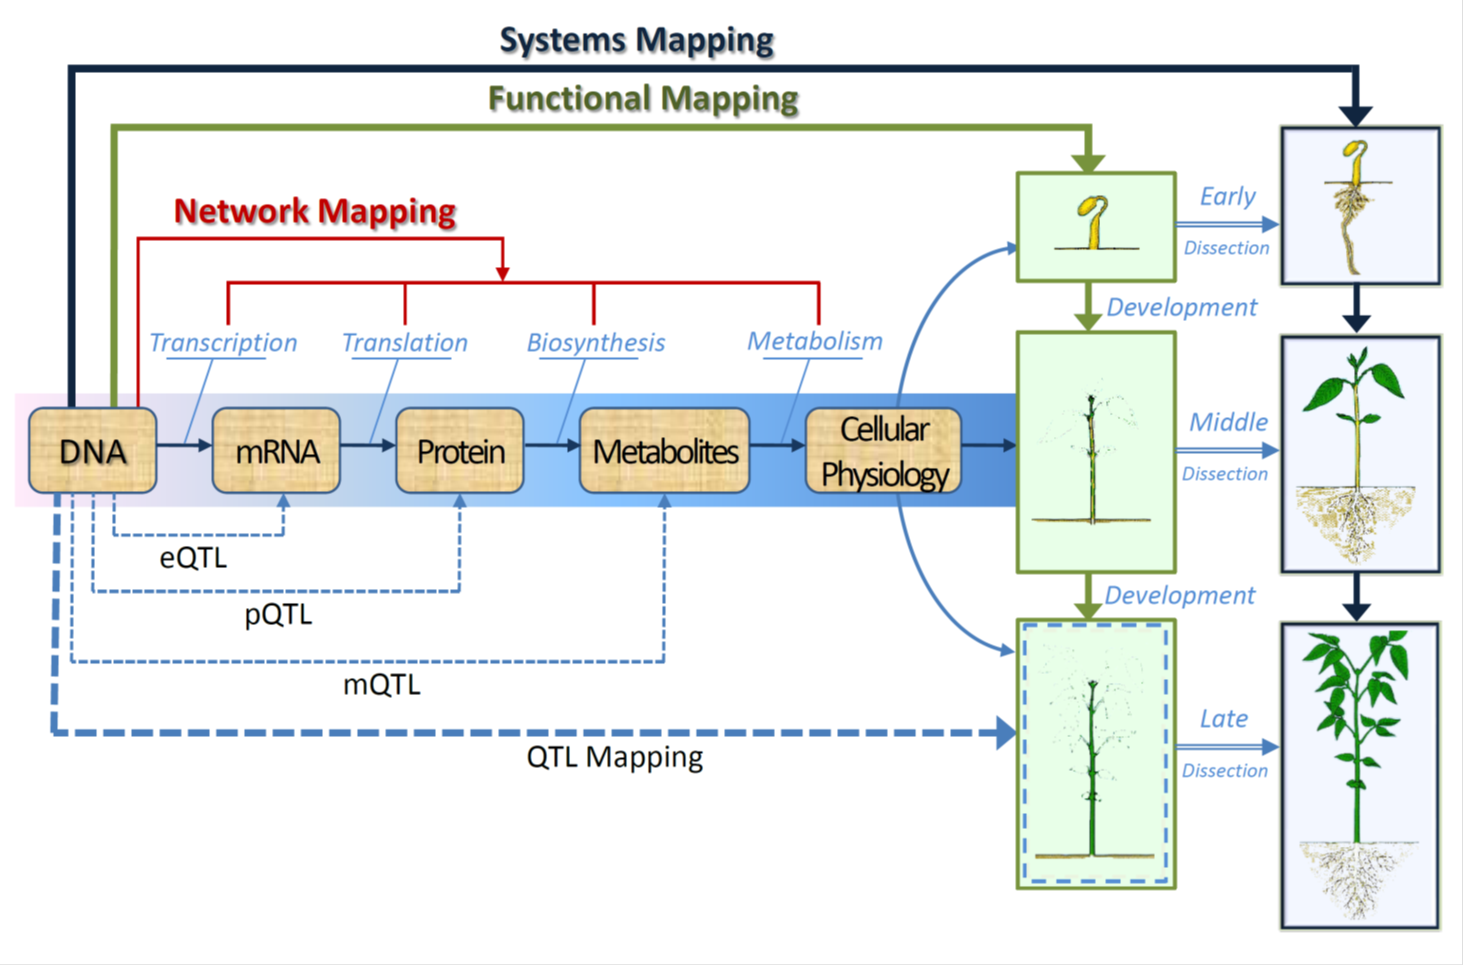
\includegraphics[width=0.8\linewidth]{images/SystemsMapping} 

}

\caption{Systems Map}\label{fig:system-map}
\end{figure}

You can label chapter and section titles using \texttt{\{\#label\}}
after them, e.g., we can reference Chapter \ref{intro}. If you do not
manually label them, there will be automatic labels anyway, e.g.,
Chapter \ref{methods}.

Figures and tables with captions will be placed in \texttt{figure} and
\texttt{table} environments, respectively.

\begin{Shaded}
\begin{Highlighting}[]
\KeywordTok{par}\NormalTok{(}\DataTypeTok{mar =} \KeywordTok{c}\NormalTok{(}\DecValTok{4}\NormalTok{, }\DecValTok{4}\NormalTok{, .}\DecValTok{1}\NormalTok{, .}\DecValTok{1}\NormalTok{))}
\KeywordTok{plot}\NormalTok{(pressure, }\DataTypeTok{type =} \StringTok{'b'}\NormalTok{, }\DataTypeTok{pch =} \DecValTok{19}\NormalTok{)}
\end{Highlighting}
\end{Shaded}

\begin{figure}

{\centering 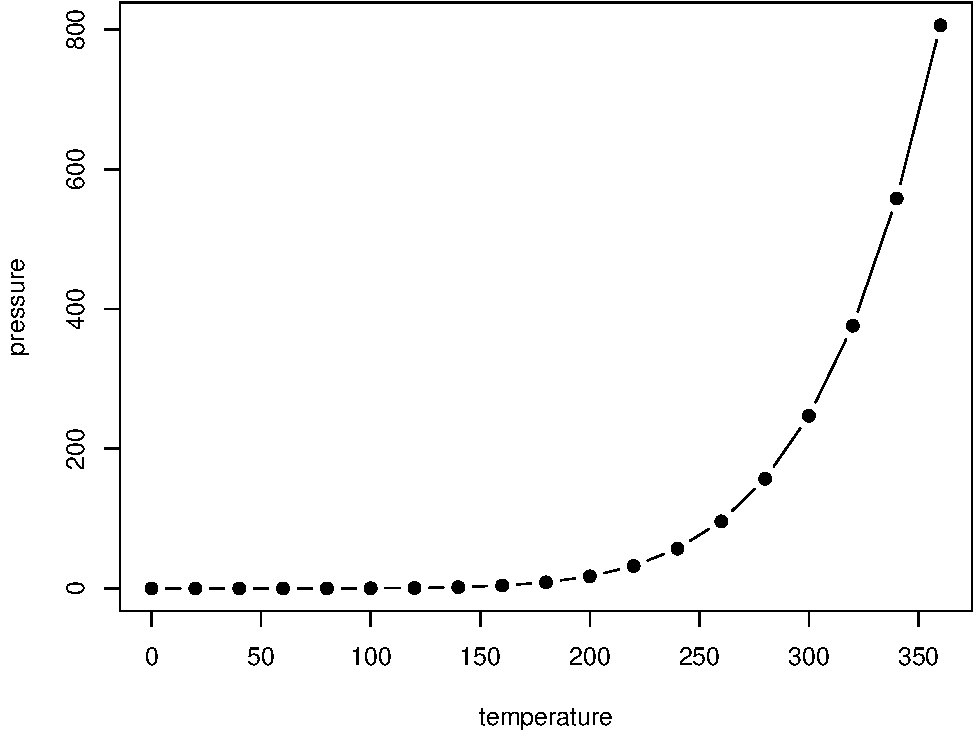
\includegraphics[width=0.8\linewidth]{Defense_files/figure-latex/nice-fig-1} 

}

\caption{Here is a nice figure!}\label{fig:nice-fig}
\end{figure}

Reference a figure by its code chunk label with the \texttt{fig:}
prefix, e.g., see Figure \ref{fig:nice-fig}. Similarly, you can
reference tables generated from \texttt{knitr::kable()}, e.g., see Table
\ref{tab:nice-tab}.

\begin{Shaded}
\begin{Highlighting}[]
\NormalTok{knitr::}\KeywordTok{kable}\NormalTok{(}
  \KeywordTok{head}\NormalTok{(iris, }\DecValTok{20}\NormalTok{), }\DataTypeTok{caption =} \StringTok{'Here is a nice table!'}\NormalTok{,}
  \DataTypeTok{booktabs =} \OtherTok{TRUE}
\NormalTok{)}
\end{Highlighting}
\end{Shaded}

\begin{table}

\caption{\label{tab:nice-tab}Here is a nice table!}
\centering
\begin{tabular}[t]{rrrrl}
\toprule
Sepal.Length & Sepal.Width & Petal.Length & Petal.Width & Species\\
\midrule
5.1 & 3.5 & 1.4 & 0.2 & setosa\\
4.9 & 3.0 & 1.4 & 0.2 & setosa\\
4.7 & 3.2 & 1.3 & 0.2 & setosa\\
4.6 & 3.1 & 1.5 & 0.2 & setosa\\
5.0 & 3.6 & 1.4 & 0.2 & setosa\\
\addlinespace
5.4 & 3.9 & 1.7 & 0.4 & setosa\\
4.6 & 3.4 & 1.4 & 0.3 & setosa\\
5.0 & 3.4 & 1.5 & 0.2 & setosa\\
4.4 & 2.9 & 1.4 & 0.2 & setosa\\
4.9 & 3.1 & 1.5 & 0.1 & setosa\\
\addlinespace
5.4 & 3.7 & 1.5 & 0.2 & setosa\\
4.8 & 3.4 & 1.6 & 0.2 & setosa\\
4.8 & 3.0 & 1.4 & 0.1 & setosa\\
4.3 & 3.0 & 1.1 & 0.1 & setosa\\
5.8 & 4.0 & 1.2 & 0.2 & setosa\\
\addlinespace
5.7 & 4.4 & 1.5 & 0.4 & setosa\\
5.4 & 3.9 & 1.3 & 0.4 & setosa\\
5.1 & 3.5 & 1.4 & 0.3 & setosa\\
5.7 & 3.8 & 1.7 & 0.3 & setosa\\
5.1 & 3.8 & 1.5 & 0.3 & setosa\\
\bottomrule
\end{tabular}
\end{table}

You can write citations, too. For example, we are using the
\textbf{bookdown} package \citep{R-bookdown} in this sample book, which
was built on top of R Markdown and \textbf{knitr} \citep{xie2015}.

\chapter{High Dimensional eQTL}\label{highdeqtl}

\section{Motivation}\label{motivation}

Since activation or inhibition of gene expression causes change in
phenotypic formation, the identification of expression quantitative
trait loci (eQTLs) that regulate the pattern of gene expression is
essential for constructing a precise genotype-phenotype map
(\cite{emilsson2008genetics}; \cite{cookson2009mapping};
\cite{nica2013expression}). With the advent and development of various
biotechnologies, it has become possible that genome-scale marker and
expression data can be generated, providing an important fuel to
systematically study the biological function of any types of cellular
components in an organism (\cite{kim2014meta}; \cite{fairfax2014innate};
\cite{lee2014common}). Several genome-wide association studies (GWAS)
have been initiated to map a complete set of eQTLs for the abundance of
genome-wide transcripts whose expression levels are related to
biological or clinical traits
(\cite{nica2013expression};\cite{li2013using};
\cite{koopmann2014genome}). Statistical analysis and modeling are
playing an increasing role in mapping and identifying the underlying
eQTLs from massive amounts of observed data
(\cite{kendziorski2006statistical}; \cite{chun2009expression};
\cite{sun2012statistical}; \cite{flutre2013statistical}).

A typical eQTL mapping approach is to associate a gene transcript with a
single marker such as single nucleotide polymorphism (SNP). By analzying
the significance of all these markers one by one adjusted for multiple
testing, one can count significant loci that contribute to variation of
expression by the gene. This marginal approach based on a simple
regression model has been instrumental for the identifcation of eQTLs in
a variety of organisms (\cite{rockman2010selection};
\cite{kim2014meta}). However, there are two major limitations for the
results by such a marginal analysis: First, it does not take into
account the dependence of different markers, thus a significant
association detected by one marker may be due to the other markers that
are linked with it. The marginal marker analysis cannot separate the
confounding effect of eQTLs due to marker-marker dependence or linkage
(\cite{wu2007statistical}). Second, an eQTL may act through its
interaction with other eQTLs and environmental factors. Because of their
paramount importance in affecting complex diseases and traits, gene-gene
interactions, or epistatic effects, and gene-environment interactions
have been studied intensively in modern biological and medical research
(\cite{cheverud1995epistasis}; \cite{moore2003ubiquitous};
\cite{van2010detection}; \cite{mackay2014epistasis})

These two limitations can be overcome by analyzing all markers and their
pairwise interactions simultaneously through formulating a
high-dimensional regression model. Although it can infer a complete
picture of the genetic architecture of gene expression, this endeavor is
highly challenged by the curse of dimensionality, i.e., the number of
predictors far exceeds the number of observations. The past decade has
witnessed the tremendous development of variable selection models for
high-dimensional data analysis, such as LASSO
(\cite{tibshirani1996regression}), SCAD (\cite{fan2001variable}),
Dantzig selector (\cite{candes2007dantzig}), elastic net
(\cite{zhao2006model}), minimax concave penalty (MCP)
(\cite{zhang2010nearly}) among others. Many methods possess favorable
theoretical properties such as model selection consistency
(\cite{zhao2006model}) and oracle properties (Fan and Lv 2011). When the
number of predictors is much larger than the number of observation, sure
screening is a more realistic goal to achieve than oracle properties or
selection consistency (\cite{fan2008sure}; \cite{wang2009forward}). Sure
screening assures that all important variables are identified with a
probability tending to one, hence achieving effective dimension
reduction without information loss and providing a reasonable starting
point for low-dimensional methods to be applied.

More recently, Hao and Zhang (\cite{hao2014interaction}) extended
variable selection approaches to jointly model main and interaction
effects from high-dimensional data. Based on a greedy forward approach,
their model can identify all possible interaction effects through two
algorithms iFORT and iFORM which have been proved to possess sure
screening property in an ultrahigh-dimensional setting. In this article,
we implement and reform Hao and Zhang's model to map the genetic
architecture of eQTL actions and interactions for gene expression
profiles. This model is modified to accommodate to the feature of a
genetic mapping or GWAS design in which molecular markers as genetic
predictors are discrete although some additional continuous predictors
can also be considered. We expand Hao and Zhang's regression model to
include discrete components. Also, for an F2 or a natural population
with three genotypes at each locus, we need to estimate a total of eight
genetic effects for a pair of markers, which are additive and dominant
effects at each locus, and additive  additive, additive  dominant,
dominant  additive and dominant  dominant effects between the two loci
(\cite{kempthorne1968correlation}). Thus, if the number of markers is p,
a total number of predictors including all main and two-way interaction
terms is \(2p^2\). For a typical moderate-sized mapping study, in which
several thousands of markers are genotyped on a few hundred individuals,
consideration of pair-wise genetic interactions will quickly make the
dimension of predictors an ultrahigh one.

By modeling all markers jointly at one time under an organizing
framework, the modified model can detect all possible significant eQTLs
and their epistasis. An eQTL can be either a cis-QTL, coming from the
same physical location as the gene expression, or a trans-QTL, coming
from other areas of the genome. Our model can more precisely discern
these two different types of eQTLs and their interactions than
traditional marginal analysis. By reanalyzing a published data collected
in a mapping population of C. elegans (\cite{rockman2010selection}), the
new model has validated previous results by the marginal approach,
meanwhile obtained new discoveries on the genetic origin of gene
expression differentiation, which could not be detected in a traditional
way.

\textbf{Add a paragraph to motivation section} Continue on about the
rest of the chapter as an overview

\section{Methods}\label{methods}

\subsection{Experimental design}\label{experimental-design}

Consider an experimental population for genetic studies of complex
traits, such as the backcross and F2 initiated from two inbred lines,
full-sib family derived from two outcrossing parents, or random samples
drawn from a natural population. These types of populations are used
specifically for different species. Although they have different levels
of complexities for statistical modeling, the genetic dissection of
different populations underlies a similar principle. For the purpose of
simplicity, we consider a backcross design in which there are only two
genotypes at each marker.

Suppose the backcross contains n progeny, each of which is genotyped by
p markers, such as single nucleotide polymorphisms (SNPs), distributed
over different chromosomes. The number of SNPs p should be large enough
to completely cover the entire genome at an adequate depth so that we
can possibly capture all possible genetic variants. An increasing body
of evidence suggests that significant SNPs associated with complex
traits or diseases are more likely to be eQTLs (\cite{li2013using}).
Hence the identification of eQTLs is an important first step toward the
genetic dissection of end-point phenotypes. For this reason, we assume
that genome-wide gene transcripts have been available for the assumed
study population. Assume that all progeny are recorded for the same
organ by microarray, leading to expression abundance data of m gene
transcripts. We purport to identify all possible genetic variants
including main effects and interaction effects of SNPs that contribute
to each gene transcript.

\subsection{Adaptation of iFORM
procedure}\label{adaptation-of-iform-procedure}

Hao and Zhang \cite{hao2014interaction} formulated an interaction
forward selecting procedure under the marginality principle (iFORM). The
marker and gene transcript data of the study population can be denoted
as \((X_i,Y_i) (i = 1, …, n)\) which are independent and identically
distributed copies of (X,Y), where \(X = (X_1,..,X_p )^T\) is a
p-dimensional predictor vector and Y is the response, expressed by a
linear regression model:

\begin{equation}
Y = \beta_0 + \beta_1 X_1 + ⋯ + \beta_p X_p + \epsilon
(\#eq: lin-mod)
\end{equation}

The 's are the coefficients for the genetic effects of each marker.
Like most genome-wide datasets, the number of markers here grossly
outnumbers the number of observations, p \textgreater{}\textgreater{} n.
Therefore, selection procedures would need to be implemented in order to
fit a linear regression model such as (1). We are already at the point
of high-dimensional data but if we want to include epistatic effects
between different markers as predictors as well it would increase the
amount of predictors by (p\^{}2+p)/2 . The resulting linear model would
grow to be,

\begin{equation}
Y = \beta_0 + \beta_1 X_1 + ⋯ + \beta_p X_p + \gamma_{11} X_1^2 +\gamma_{12} {X_1}{X_2} + ⋯ + \gamma_{pp} X_p^2 + \epsilon
(\#eq: lin-mod2)
\end{equation}

where 's are the coefficients for the epistatic effects for all the
quadratic and two-way interactions between the markers. For convenience
we will assume that the markers and the transcripts are standardized
before running the selection procedure. Therefore, E(X\_ij )=0,Var(X\_ij
)=1,E(Y\_i )=0 and Var(Y\_i )=1 for i=1,\ldots{},n; j=1,\ldots{},p.
Also, the quadratic and two-way interaction effects will be centered
which we will write as Z\_i=(\ldots{},X\_ik X\_il-E(X\_ik X\_il
),\ldots{})\^{}T. By doing so we would eliminate the need for an
intercept in regression model (2). This would reduce the model to the
form,

\begin{equation}
Y = X^T \beta + Z^T \gamma
(\#eq: lin-mod3)
\end{equation}

Some notations that will be used to define the elements of
\cite{hao2014interaction} iFORM procedure are as follows.\\
\(P_1 = {1,2,…,p}\) \(P_2 = {(k,l):1 ≤ k ≤ l ≤ p}.\) which are the index
sets for the linear and two-way interactions terms, respectively. The
significant main effects for the markers and their interaction effects
are
\(T_1 = {j:\beta_j \ne 0,j\in P_1},T_2 = {(j,k):\beta_{jk} \ne 0,(j,k) \in P_2 }.\)
For any model M, \textbar{}M\textbar{} will be used to denote the number
of predictors contained in the model. The true model size would be
indicated by \(|T_1| = p_0\) and \(|T_2| = q_0\) or together would be
\textbar{}T\textbar{}=d\_0=p\_0+q\_0. For the procedure, three sets will
be used throughout. The sets are M for the model set, C for the
candidate set of predictors and S for the solution set of predictors
currently selected in the model.

There are two principles that are used in the selection procedure when
considering interactions as candidates for selection into the final
model. The first is considering the principle of marginality. The
principle states that it is inappropriate to model interaction terms
when the main effects contributing to the interaction have either not
been included in the model or are deleted because their effects become
marginal by the inclusion of the interaction effect. The second
principle important to the procedure is the heredity principle. The
strong case of the principle states that an interaction effect should
not be considered unless both the contributing main effects are in the
model (\cite{zhao2006model}). This would translate to
\(\gamma_{jk} ≠ 0 only if \beta_j, \beta_k \ne 0 \forall 1 ≤ j, k ≤ p\)
for model (2). By including both principles during the selection process
it allows for dynamically including both main effects and interactions
effects. The interaction effects can only be considered between the main
effects currently selected into the solution set of the model according
the discussed principles. A more formal description of the procedure is
given below.

\subsection{iFORM}\label{iform}

\cite{hao2014interaction} formulated an interaction forward selecting
procedure under the marginality principle (iFORM). The procedure's
initial step starts with the empty set for both the solution set and the
model set, \(S_0=\emptyset\) and \(M_0=\emptyset\). The candidate set
contains all main effects at the beginning, \(C_0 = P_1\), for each of
the markers as a possible eQTL. Typical forward selection procedures are
carried out to start the selection. Each marker is tested individually
using a marker regression. The marker that results in the lowest
residual sum of squares is the marker selected from the candidate set
into the solution set as an eQTL. This is then iterated again for a
selection of another marker into the model set. Once there are at least
two main effects selected into the solution set, using the strong
heredity principle, the quadratic and two-way interactions are then
created and placed into the candidate set as possible eQTLs for
selection in the next step. This process continues selecting main
effects or the newly created interaction effects into the solution set.
If another main effect is selected into the solution set, then the
candidate set grows with the creation of all possible two-way
interactions of the main effects that are currently in the solution set.
This is continued until a designated stopping value, say d. For the
number of predictors placed into the model set from the solution set the
Bayesian information Criterion was used,
\(BIC_2(\hat M)=log(\hat \sigma \hat M)+n^{-1} |\hat M|\star(log(n)+2\star log(d^\star))\),
where \(\sigma^2 \hat M\) is the sample variance for the given model,
\(|\hat M|\) is the size of the model or the number of predictors
selected into the given model, and n is the sample size. The \(d^*\)
term is the number of predictors in the full model. This was proposed as
\(BIC_2\) by \cite{chen2008extended} which they derived to help control
the false discovery rate in high dimensional data situations. They also
showed that it was selection consistent if \(d^\star = O(n^\xi)\) for
some \(\xi > 0\). The only difference between the traditional \(BIC\)
calculation and the \(BIC_2\) is the additional term involving
\(2log(d*)\). Ignoring the \(BIC\), the most the number of steps in the
solution path is of size n. The parameter d controls the overall length
of the solution path. In practice, the exact number of predictors to
include, say d\_0, in the true model is unknown. We want to make d large
enough to include d\_0 but not so large as to fit the model to the point
where it becomes oversaturated. Using the \(BIC_2\) should help avoid
such a matter as well. It is reasonable to assume that d\_0 is much
smaller than n in high dimensional sparse regression problems
(\cite{fan2008sure}). Since this is the case, for the purposes of our
model, d was set to be no larger than \(n/loga(n)\). Generally, the
\(BIC_2\) should reach minimum, indicating the optimal stopping point,
before the designated stopping value, is reached.

\subsection{Some considerations}\label{some-considerations}

There were some considerations and pre-processing steps taken before the
iFORM procedure was implemented. The first consideration was to see if
there were any exact duplicate markers in the dataset. One drawback that
could arise with marker datasets when attempting to run multiple linear
regression is the possibility of duplicate markers in the dataset. If
two different markers would happen to have exactly the same genotypes
for each subject it would show up as an exact linear combination of each
other if both markers were to be placed in the linear model. Including
redundant markers in a linear model would not add any additional
information and therefore should not be included in the candidate set
during the selection procedure. This also reduces the dimension slightly
when there are duplicate markers in the dataset.

Another consideration made is the type of coding used for the genotypes.
At any given eQTL, the jth eQTL, say, there are two possible genotypes:
Q\_j Q\_j and Q\_j q\_j, making the total number of possible QTL
genotypes in the population 2\^{}m. The goal of a genetic model is to
relate the 2\^{}m possible genotypic values to a set of genetic
parameters, such that these parameters are interpretable in terms of
main and epistatic effects of the m eQTL. A genetic model is to use
orthogonal contrast scales because it is consistent in the sense that
the effect of a eQTL is consistently defined whether the genetic model
includes one, two, three, or more eQTL (\cite{kao2002modeling}). The
orthogonal contrasts for the genetic model can be expressed by
\(x_{ij} = \left[\frac{-1}{2} if homozygote Q_j Q_j, \frac{-1}{2} if heterozygote Q_j q_j \right]\)
Typically in an inbred line backcross population a given genotype is
coded with a 0 and 1. However there are two draws backs to this coding
when considering the selection procedures discussed above. The first
issue comes with not including an intercept in model (2). If this is the
case each of the predictors would need to be centered making the coding
to -1/2 and 1/2 instead of 0 and 1. Besides meeting the assumptions of
the model that the predictors are centered, it is also beneficial for
the interaction effects as well. If the coding would remain at 0's and
1's, the interaction coding would also consist of 0's and 1's. This
could propose a problem because three out of the four scenarios of
epistasis between markers would result in a coding of 0 for the level in
the interaction effect. This has the potential to falsely skew the data
of no additive effect for interactions terms because of the sparseness
of coding. By centering the coding to \((-1/2,1/2)\), it would result in
an interaction effect being coded as \((-1/4,1/4)\). This coding would
happen for different scenarios for each of the levels. The -1/4 could
arise when the interaction is made up of a homozygote interacting with a
heterozygote genotype. A coding of 1/4 would arise by either a
homozygote interacting with another homozygote genotype, or when a
heterozygote interacts with another heterozygote genotype.

\section{Application}\label{application}

\subsection{Simulation Results}\label{simulation-results}

Simulations studies were conducted to test the theoretical properties of
the selection procedures and the results \textbf{(Tables 1
-3)\ref{tab:nice-tab}}. The results were compared to several other
commonly used methods for eQTL mapping. In each of the examples the
response was generated from model (2) with σ=1,2,and 3 for the random
error with a sample size of \(n=200\). The \(X_i\)'s were all
independently and identically distributed realizations generated from
\(Binomial(0.5)\) and then orthogonal contrasts were made making each
\(x_ij∈(-1/2,1/2)\). The true \(β=(〖3,0,0,3,0,3,3,0〗_493)\), therefore
making \(T_1={1,4,6,7}\) and \(p_0=4\). The relevant interactions were
set to the pairs \(T_2={(1,6),(1,7),(4,7),(4,7)}\) and \(q_0=4\) all
with \(γ_jk=3\) where \((j,k)∈T_2\). There were several methods compared
during each of the simulations \textbf{(Tables 1 -3)\ref{tab:nice-tab}}.
The methods that were used to model the data were single marker
analysis, forward selection involving only main effects (FS), forward
selection involving all main effects and interaction (FS2) and the iFORM
procedure. Several outcomes were evaluated to compare across each of the
models. The outcomes are separated into three parts. The first part
focuses on the selection of main effects, the second part focuses on the
selection of interaction effects and the third part is the overall model
performance. Simulations of M=100 replicates were run and the outcomes
considered include

\emph{Convergence Probability (Cov) \(∑_(m=1)^M▒〖I(T⊂T ̂ )/M〗\)
}Percentage of correct zeros (Cor0)
\(∑_(m=1)^M▒∑_(j=1)^p▒〖I((β_j ) ̂=0,β_j=0)/[M(p-p_0)]〗\)
\emph{Percentage of incorrect zeros (Inc0)
\(∑_(m=1)^M▒∑_(j=1)^p▒〖I((β_j ) ̂=0,β_j≠0)/[M(p_0)]〗\) }Exact Selection
probability (Exact) \(∑_(m=1)^M▒〖I(T=T ̂ )/M 〗\) \emph{The average
model size }Mean Square Error (MSE) \emph{Adjusted R-square }Computation
Time in seconds

In each instance of the simulation, the iFORM procedure was closest to
the simulated data, indicated as Oracle. Single marker analysis was
conducted on each of the main effects individually and the significant
markers were then designated as eQTLs. When comparing the single marker
analysis, we can see it rarely designated the full set of main effects
as significant from the simulated data. Also, no consideration for
interactions could be assessed in single marker analysis. The iFORM
procedure contains the identified main effects over 90\% of the time
across all simulations. The procedure also includes interaction
selection. The interaction screening shares a similar success rate where
the interaction effects are correctly selected over 90\% of the time as
well. Focusing on the computation time, we observed only a few seconds,
on average, increase than running single marker analysis. The final
models selected by the iFORM procedure had similar adjusted R-square
values as the Oracle results, on average. Looking at the exact selection
percentage, we can see that the vast majority of the time the correct
predictors were selected and indicated as significant each time. To
compare the interaction screening effectiveness, forward selection was
implemented on both the main effects and interactions effects. The time
it took to create the design matrix in order to implement forward
selection was not included in the computation time. As can be seen from
the results, using forward selection on the full set of main effects and
pair-wise interactions took substantially longer to run on average than
any of the other methods, including the iFrom procedure. Another
drawback to implementing forward selection on such a large set seemed to
come with over fitting the model. The selection included the maximum
number of predictors allowed by the designated stopping value and did
not use the BIC criteria for final model selection. This resulted in 19
additional predictors selected \textbf{(Tables 1 -3)\ref{tab:nice-tab}}.
This increased the adjusted R-square value of the final model, however
this is suspected because of over fitting the data and not to be a true
prediction of the response.

\subsection{Real Data Analysis}\label{real-data-analysis}

\cite{rockman2010selection} reported an eQTL mapping study of C. elegans
using 208 recombinant inbred advanced intercross lines (RIAIL) from a
cross between the laboratory strain, N2, and a wild isolate from Hawaii,
CB4856. Abundances of 20,000 gene transcripts were measured by
microarray in developmentally synchronized young adult hermaphrodites of
these lines, providing a genome-wide coverage of C. elegans from
WormBase, a public C. elegans genome database. The microarray data was
preprocessed through a normal--exponential convolution background
correction and normalized using quantile standardization. Although they
are closely related, the two strains used for the cross are considered
relatively divergent for C. elegans. The two strains differ roughly at
approximately 1 base pair per 900. Their RIAILs were genotyped at 1454
ordered single-nucleotide polymorphism (SNP) markers that cover the
whole genome of C. elegans including five autosomes (denoted as I -- V)
and one sex chromosome (denoted as X).

\cite{rockman2010selection} used a classic interval mapping approach to
detect 2309 eQTLs by testing and scanning associations of each SNP with
each gene transcript over the entire genome. Rockman et al.'s analysis
allowed a rectangular map of eQTL positions  gene positions to be
constructed (Fig. 1), from which one can identify cis-eQTLs on the
diagonal and trans-eQTLs off the diagonal. However, because their
association analysis was conducted individually for each SNP, the
detection of eQTLs was based on the marginal effects of individual
eQTLs, which may lead to two issues being unsolved. First, of those
eQTLs detected for the same gene transcript, some may include confounded
effects by others. Second, the effects of genetic epistasis may take
place but were not detected. By analyzing all SNPs simultaneously under
a single framework, the high-dimensional model, iFORM, implemented in
this study can more precisely characterize the genetic machineries
underlying variation in each gene transcript. More specifically, we
treat each transcript as a response with all SNP markers and their
interactions as predictors by building a big regression model.
Significant predictors were then selected based on the iFORM procedure.
A final model including both main and interaction effects can be
evaluated by calculating adjusted R-square values

Figure 2 illustrates the map of how a particular gene transcript is
controlled by its eQTLs through main effects and interaction effects.
For clarity of our presentation, we only chose one representative gene
transcript from each chromosome. For example, gene transcript
A\_12\_P103290 located at position 2069088 -- 2069147 of chromosome I
was detected to be controlled by main effects due to X2\_13516256 eQTLs
on chromosomes II and X4\_15632637 eQTLs on chromosome IV and
X2\_13516256:X4\_15632637 interactions between some of these eQTLs on
these two chromosomes.

iFORM provides the estimates of each effect (either main effect or
interaction effect), standard errors of each estimate and the
significance tests of each effect. As an example, Table 4 gives the
result of how gene transcript A\_12\_P103290 can be predicted by its
eQTLs and their interactions. It can be seen that the final predictive
model (adjusted R2 = 0.896) contains 14 markers which exert their main
effects and/or interaction effects on the transcript. Of the 14 final
markers, a half shows significant main effects (p \textless{} 0.05),
with several (i.e., X\_14636404, X4\_15568674, X4\_15632637 and
X\_14542103) explaining about 5\% heritability (defined as a proportion
of genetic variance due to a predictor over the total phenotypic
variance). Of these final markers, we identified eight significant
epistatic interactions. Each epistasis accounts for 4.6 -- 5.5\%
heritability (Table 4).

It is interesting to note that all predictors jointly contribute to
62.6\% heritability for transcript A\_12\_P103290, of which main effects
account for 26.7\% and epistatic effects account for 35.9\%. It is very
surprising that epistasis contributes to more than a half of
heritability. Of the eight epistatic interactions, only one occurs due
to the interaction between two significant eQTLs, X\_14542103 and
X4\_13532205 (Table 4). All the remaining is due to interactions between
one significant eQTL and one non-significant marker. Some eQTLs, such as
X\_14542103 and X\_14636404, produce epistasis with a greater frequency
than others. Despite their involvement in the final predictive model,
some markers were tested to be insignificant in terms of both main and
interaction effects, suggesting that they regulate a gene transcript in
a subtle but important fashion. In summary, iFORM can not only provide
an estimate of the overall heritability of gene transcript
A\_12\_P103290 (i.e., the sum of individual heritabilities explained by
each predictor), but also chart a detailed picture of how each genetic
variant contributes to transcript variation. In particular, iFORM can
characterize epistasis and its role in trait control, thus equipped with
a capacity to retrieve so-called missing heritabilities
(\cite{manolio2009finding}), a significant issue arising from current
genome-wide association studies.

Through analyzing associations between all markers and each transcript
by iFORM, we can identify the difference of cis- and trans-eQTLs for a
particular transcript. For example, of the eQTLs affecting
A\_12\_P103290, we detected that X1\_2068168 is a cis-eQTL, whereas all
others are trans-eQTLs (Table 4). We list the number and distribution of
these two types of eQTLs and the pattern of how they interact with each
other to determine gene transcripts (Table 5). By detecting cis-eQTLs
and trans-eQTLs, iFORM detected that genetic interactions take place
mostly between trans-eQTLs.

\section{Discussion}\label{discussion}

With the recent development of genotyping and sequencing techniques, the
collection of genome-wide genetic and genomic data from any tissue of an
organism has been made much easier and more efficient. Because of this,
genetic studies of complex diseases or traits have developed during the
past decade to a point at which we can draw a complete picture of
genetic architecture for disease or trait formation and progression by
genome-wide association studies (GWAS) (Mackay et al. 2009). Traditional
marginal analysis based on simple regression has been instrumental for
the detection of important genetic variants or quantitative trait loci
in a variety of organisms, but its bottleneck has emerged quickly due to
its limitation in precisely and comprehensively charting genetic control
landscapes. Many GWAS studies published are bothered by missing
heritabilities because of their incapacity to detect genome-wide
epistasis and genotype  environment interactions
(\cite{manolio2009finding}).

Epistasis is a phenomenon by which the influence of a gene on the
phenotype depends critically upon the context provided by other genes
(\cite{cheverud1995epistasis}). It has been increasingly recognized that
epistasis is an important source for trait variation
(\cite{moore2003ubiquitous}; \cite{carlborg2004epistasis};
\cite{cordell2009detecting}), thus inclusion of epistasis would enhance
the prediction accuracy of phenotypic performance and shed more light on
the global genetic architecture of trait control (Mackay 2014). However,
epistasis is extremely hard to detect as an interaction term, whose
inclusion may complicate the inference of the predictive model
(\cite{carlborg2004epistasis}; \cite{mackay2014epistasis}). Thanks to
recent progresses in high-dimensional data modeling, we have been able
to implement several cutting-edge statistical models for systematical
detection and characterization of genome-wide epistasis.

\cite{hao2014interaction} proposed a new high-dimensional model, iFORM,
that can tackle an issue of interaction selection simultaneously from a
large pool of continuous predictors. This model is based on
forward-selection-based procedures, characteristic of computational
feasibility and efficiency. The authors further proved that the
detection of interactions by iFORM is consistent, even if the dimension
increases exponentially for a sample size. As one of the first attempts
to introduce high-dimensional models into genetic studies, we modified
iFORM to accommodate to the discrete nature of molecular markers. Our
simulation studies indicate that iFORM can provide reasonably accurate
and precise estimates of genetic main effect and interaction effects.
Also, it shows greater power to detect significant genes and their
interactions which may not be detected by traditional single marker
analysis.

We applied iFORM to re-analyze gene expression data in an eQTL mapping
study (\cite{rockman2010selection}). While our results confirmed those
by the traditional approach, the new model provides some new findings
including new eQTLs and epistasis, thus allowing a complete set of
genetic variants to be characterized. As an important tool to understand
the genetic mechanisms underlying both complex traits and diseases, eQTL
mapping has been widely used to identify key regulatory pathways toward
endophenotype and end-point phenotypes (\cite{schadt2005integrative};
\cite{emilsson2008genetics}; \cite{cookson2009mapping};
\cite{pickrell2010understanding}; \cite{nica2013expression}). A typical
eQTL study may not only include a large number of molecular markers as
like in a GWAS, but also record tens of thousands of gene transcripts
throughout the entire genome. Our current version of iFORM can only take
into account one gene transcript as a response at a time, thus having a
limitation to model the correlation and dependence among different
genes. It is our next step to formulate a multivariate multiple
regression model by which to test how an individual predictor, main
effect or epistatic effect, pleiotropically affects correlated
expression profiles of different genes.

Given the complexity of biological phenomena, pair-wise epistasis may be
insufficient to explain phenotypic variation.
\cite{imielinski2008exploiting} argued that high-order interactions
among more than two genes may provide a key pathway toward complex
traits. Three-way interactions have been detected in trait control
(\cite{mcmullen1998quantitative}; \cite{stich2007power}). A model for
modeling three-way interactions has been developed in a case-control
GWAS design (\cite{wang2010general}) and a genetic mapping setting
(\cite{pang2013statistical}). It is crucial to extend iFORM to map main
effect, two-way epistasis and three-way epistasis in an eQTL mapping
study although no substantial change is needed in the computational
algorithm, except for an enlarged test set and extra computing time. Our
work is based on a backcross population in which there are only two
genotypes at a locus. The backcross population can facilitate our
estimation and test of genetic effects owing to a smaller number of
parameters at each locus or locus pair, but its utility is very limited
in the F2 design of model systems and natural populations of outcrossing
species such as humans. A more general model of iFORM should consider
three genotypes at each locus, which provides estimates of additive and
dominant effects at each locus and four types of epistasis, i.e.,
additive  additive, additive  dominant, dominant  additive and
dominant  dominant, between each pair of loci
(\cite{kempthorne1968correlation}). Each of these epistatic types may
affect a phenotype through a different pathway.

With continuous falling of sequencing price, we will have desirable
opportunities to study the dynamic behavior and pattern of gene
expression profiles across time and space scales
(\cite{vinuela2010genome}; \cite{ackermann2013impact}). Many previous
studies suggest that gene expression during cell and organ development
may follow a particular form, which can be quantified by mathematical
equations (\cite{kim2010wavelet}). For example, abundance of gene
expression may change periodically in human's brain during circadian
clock. Many researchers used Fourier's series approximation to model the
periodic changes of gene expression by estimating the period and
amplitude of the cycles (\cite{li2013using}). By integrating Fourier
series into iFORM, we will be able to map dynamic eQTLs for gene
expression and make a quantitative prediction of temporal and spatial
patterns of genetic control by eQTLs.

\chapter{High-order Epistatic Networks}\label{highorder}

\section{Motivation}\label{motivation-1}

\textbf{Shoot-Root Manuscript} Following Sun et al.'s
\cite{sun2014model} developmental model, we calculated and chose four
key heterochronic parameters, asymptotic growth (a), relative growth
rate (r), the timing of inflection point (TI), and the duration of
linear growth (L), as phenotypic values to perform QTL mapping. A great
variability was observed for growth curve parameters of both phenotypic
traits (Table 1). Compared with taproot length, shoot length has a
greater rate of growth and reaches the maximum growth rate at an earlier

\textbf{Start of My Paper}

Quantitative traits are very difficult to study because these traits are
controlled by many genes that interact in a complicated way
(\cite{nelson2013century}; \cite{mackay2014epistasis}). Genome-wide
mapping and association studies increasingly available due to
next-generation high-throughput genotyping techniques have proven to be
useful for characterizing gene-gene interactions, coined epistasis, that
contribute to phenotypic variation (\cite{cordell2009detecting};
\cite{van2011travelling}; \cite{wei2014detecting}). Powerful statistical
methods have been developed to analyze all possible markers
simultaneously, from which to search for a complete set of epistasis for
quantitative traits (\cite{li2014fast}; \cite{gosik2016iform}). The
joint analysis of all markers is particularly needed to chart an overall
picture of genetic interactions, in comparison with computationally less
expensive marginal analysis.

Epistasis reported in the current literature is mostly due to
interactions between two genes. However, a growing body of evidence
shows that genetic interactions involving more than two loci play a
pivotal role in regulating the genetic variation of traits
(\cite{wang2010general}; \cite{dowell2010genotype};
\cite{pang2013statistical}; \cite{taylor2014genetic}). For example, in a
mapping population deriving from crossing two chicken lines, three-locus
interactions were detected to determine body weight
(\cite{pettersson2011replication}). A mapping study established by two
yeast strains identified genetic interactions involving five or more
loci for colony morphology (\cite{taylor2014genetic}). Other studies
have demonstrated that high-order epistasis is of critical importance in
regulating metabolic networks in yeast (\cite{weinreich2013should}) and
Escherichia coli and Saccharomyces cerevisiae
(\cite{imielinski2008exploiting}; \cite{he2010prevalent}), whereas
lower-order (pairwise) epistasis may be insufficient to explain
metabolic variation for these organisms.

The theoretical models of high-order epistasis have well been
established by mathematical biologists (\cite{hansen2001epistasis};
\cite{beerenwinkel2007analysis}). These models provided a foundation to
interpret high-order epistasis from a biological standpoint. A few
statistical models have been derived to estimate and test high-order
epistasis in case-control designs (\cite{wang2015bayesian}) and
population-based mapping settings (\cite{pang2013statistical}).
\cite{wang2015bayesian} developed a Bayesian version of detecting
high-order interactions for both continuous and discrete phenotypes.
However, these models were based on a marginal analysis, thus less
powerful to illustrate a global view of genetic control mechanisms due
to high-order epistasis.

In this article, we deploy a variable selection procedure within a
genetic mapping or association setting to characterize the genetic
architecture of complex traits composed of main effects of individual
genes, pairwise epistasis between two genes, and three-way epistasis
among three genes. The model was built on greedy interaction screening
forward selection developed under the marginality principle (named
iFORM) by \cite{hao2014interaction}. These approaches, proved to possess
sure screening property for ultrahigh-dimensional modeling, have been
implemented to model the genetic architecture of main effects and
pairwise epistasis due to eQTLs for gene transcripts
(\cite{gosik2016iform}). Here, we extend the implementation of iFORM to
systematically capture three-way interactions that are expressed among
all possible markers studied. To show the statistical power of the
extended model, we performed computer simulation studies. The model was
further validated through analyzing a real data of genetic mapping for
shoot growth in a woody plant, mei (Prunus mume). The model should be
used in any other mapping or association studies of quantitative traits.

\textbf{Add a paragraph to motivation section} Continue on about the
rest of the chapter as an overview

\section{Methods}\label{methods-1}

\subsection{Mapping and association
studies}\label{mapping-and-association-studies}

Genetic mapping and association studies are two types of designs used to
dissect quantitative traits. The former is based on a controlled cross
derived from distinct parents, whereas the latter samples different
genotypes from a pool of accessions or a natural population. In both
types of design, a set of individuals are sampled to be phenotyped for
quantitative traits of interest and genotyped by molecular markers
distributed throughout the entire genome. For a particular genetic
experiment, the number of markers is much larger than that of samples,
thus, it is impossible to estimate the genetic effects of all markers
simultaneously using traditional regression models. This issue becomes
much intractable when we aim to estimate genetic interactions of
different orders. To tackle the issue of the number of predictors
\textgreater{}\textgreater{} the number of samples, several variable
selection approaches have been implemented in association studies. One
approach is forward selection which was shown to be robust for
estimating pairwise interactions of predictors (Hao and Zhang 2014).
With sure screening properties and controlling for false positives, this
approach, named iFORM, performs very well in capturing important
information in explaining the response variable. On top of these nice
theoretical properties it is computationally efficient by using ordinary
least squares calculations and only requiring a predetermined set up
steps. Here, we extended the iForm procedure to include HGI's to capture
more relevant information. In the following sections, the notation and
model set-up will be introduced. After this theoretical properties will
be explored. Finally simulated and real data analysis will be conducted
to help confirm the theoretical properties and show the feasibility of
using the model for screening across whole genomes to more precisely
explain phenotypes of interest.

\subsection{Epistatic model}\label{epistatic-model}

Consider a linear model that underlies the true genotype-phenotype
relationship. Assume that the phenotype, as the response of the model,
is controlled by a set of p SNPs that act singly and/or interact with
each other. These main and interaction effects of markers, i.e., the
predictors of the model, need to be estimated. Let \(Y = (y1, …, yn)^T\)
denote the phenotypic value of n samples from a mapping or association
population. When considering pairwise and three-way interactions, the
linear model is expressed as

\begin{equation}
Y = \alpha + X^T\beta + Z^T\gamma + W^T\eta + \epsilon
\label{eq:lin-mod}
\end{equation}

where \(X=(X_1,…,X_p )^T\) is the design matrix that specifies the
genetic effects of each
\(marker  = (1, …, p) , Z=(X_j X_k )^T (1≤j≤k≤p)\) is the design
matrix that specifies the epistatic effects between two markers,
expressed in \(\gamma, W=(X_j X_k X_l )^T (1 ≤ j ≤ k ≤ l ≤ p)\) is the
design matrix that specifies the epistatic effects among three markers,
expressed in \(η\), and \(\epsilon ~ N(0,\sigma^2 )\) is the residual
error normally distributed with mean zero and variance σ\^{}2. We denote
the index sets for the linear, order-2 and order-3 effects in equation
(1), respectively, as \(P_1={1,2,…,p}\) \(P_2={(j,k):1≤j≤k≤p}\)
\(P_3={(j,k,l):1≤j≤k≤l≤p}\) With the significant main, order-2
interaction and order-3 interaction effect sets being,
\(T_1={j:β_j≠0,j∈P_1 }\) \(T_2={(j,k):γ_jk≠0,(j,k)∈P_2 }\)
\(T_3={(j,k,l):η_jkl≠0,(j,k,l)∈P_3 }\)

The true size of \(T_1\), will be \(p_1\) and similarly for \(T_2\) and
\(T_3\) will have sizes \(p_2\) and \(p_3\) respectively. There will be
a total of 3 sets referred to throughout the procedure, the candidate
set \(C\), the selection set \(S\) and the model set, \(M\). The
candidate set is the set of all possible predictors at a given step in
the selection process. The selection set contains the predictors that
have previously been selected from the candidate set from each iteration
of the procedure. Finally, the model set is the final model that is fit
from the selection set at the end of the procedure. The BIC is used to
determine the optimal cutoff for the final model size.

\subsection{iForm with high-order
epistasis}\label{iform-with-high-order-epistasis}

The iForm procedure is a forward selecting procedure. In traditional
forward selection the procedure starts with the empty set and then
iterates through the entire set of possible predictors in \(C\) and
selects the best predictor and includes it in S at the end of each step.
The best predictor can be determined in many ways but usually is defined
by the predictor that results in the least amount of error. For our
purposes we use the residual sum of squares. This continues with
selecting the best predictor from C at each step until a designated
stopping criterion is met or until some information criterion is met.
Common information criteria used for selecting predictors to be in \(M\)
are AIC, BIC, \(R^2\) and Mallow's \(C_p\) statistic.

The iForm procedure for high-order epistatic detection parallels the
forward selection procedure, but C will grow dynamically with the
creation of order-2 and order-3 interaction effects between main effects
that were included from previous iterations of the procedure. There are
three steps to the model selection. The first step is to initialize the
3 sets mentioned above. The sets, \(S\) and \(M\) are set to the empty
set while the candidate set, \(C\), is first set to \(P_1\), all the
main effects. The next step starts the forward selection procedure
selecting predictors from \(C\). The selected predictor will be a main
effect at the first step. At subsequent steps, after interaction effects
are included, selected predictors could be either be a main effect,
order-two or order-three interaction effect. The final step involves
repeating the second step until a designated stopping criterion is met.
This can be a certain amount of predictors to be considered in the final
model, or it can be based off of other factors such as the sample size.
The designated stopping criterion will be denoted as d. For our purposes
we use d as a function of the sample size, \(d = n/lo g_2a(n)\). The
procedure will run up until d iterations, and the optimal model will
then be constructed from the selection set. This is done by an
information criterion. Here we used the Bayesian Information Criterion
proposed by \cite{chen2008extended} denoted as the \(BIC_2\). This was
derived by them to control the false discovery rate in high dimensional
model selections.

\begin{equation}
BIC_2(\hat{M}) = log(\hat{σ_M}^2) + n^{-1} |\hat{M}| * (log(n) + 2*loga(d^*))
\label{eq:bic2}
\end{equation}

Once the selection procedure is done and there are d predictors in the
selection set the BIC is used to determine the cutoff value for the
optimum number of predictors in the model set. Then linear regression is
performed on the model set.

Two guiding principles are used to help dynamically select the main
effects and epistasis effects throughout the procedure. The first is the
marginality principle, which states that an effect will not be removed
from the model once it has been selected. A previous selected effect may
become marginal by the inclusion of subsequent effects. This especially
can be the case when an interaction effect is included. One of the
parent effects may become less significant or even not significant at
all by considering both in the model. The next principle we state as the
heredity principle but has also been referred to in other work as the
hierarchy principle (Bien et al 2013 and Lim and Hastie 2014).

The heredity (hierarchy) principle help reduce the search space by
making the assumption that previously selected main effects would be
involved in the interaction effects. By considering this principle it
substantially reduces the search space making this feasible for
ultra-high dimensional situations. Even larger than ram datasets can be
used with efficient memory mapping of the dataset while running the
procedure. The weak version of the heredity principle for three-way
interactions states that at least one of the main effects needs to be
selected into the model to consider an interaction effect that contains
that predictor. Considering a moderately high set of predictors say p =
5000, if trying to include all order-2 interactions upfront, will make
the candidate set be as high as 12,498,000. This alone could exceed most
ram requirements of standard computers. This is before even stepping up
to order-3 interactions. The weak heredity principle would decrease the
candidate set substantially. Assuming a sample size of \(n = 200\),
would give a cut off of \(n/log_{2}(n) = 200/log_{2}(200) = 26\) steps
in the procedure. This would give a maximum of approximately 135,000
candidate predictors. This gives a 100 fold decrease in the candidate
set. This could substantially make ultra-high dimensional analysis more
feasible and also speed it up in the process. This is the weak case. If
considering the strong case the decrease in candidate space is even more
apparent. Aside from the efficiency by lowering the search space of the
candidate set, the heredity principle is usually taken into account by
researchers when selecting models involving the consideration for
interaction effects.

\subsection{Theoretical Properties}\label{theoretical-properties}

The theoretical properties of the iForm procedure with high-order
epistasis follow closely with the forward selection procedure.
\cite{hao2014interaction} summarize forward selection nicely as follows.
At each step, the response is regressed on the most correlated
covariate, and the residual is calculated and used as the new response
in next step. After the most correlated covariate (say, \(X_1\)) is
selected, all other covariates are regressed on \(X_1\), and then the
covariates are substituted by the corresponding normalized residuals,
which are used as the new covariates in next step. By viewing forward
selection in this sense the computational complexity of the procedure
depends upon the size of the candidate set. The candidate set in the
iForm's case does grow dynamically at each step, by at most the number
of predictors currently selected in C for each step. If we denote the
current size of the candidate set as m then each iteration of the
procedure grows with complexity of O(nm), where n is the sample size.
Leaving the selection unrestricted we would not be able to fit more than
n predictors for a linear model and therefore n would be the most main
effects that would be able to be selected. Considering the weakest form
of the heredity principle at the current iteration there would be at
most \(p + (n(n-1)(n-2))/6\) predictors in the candidate set. This would
make the total complexity of the selection procedure to be
\(nO(n(p+n(n-1)(n-2))) = O(n^3 p+n^5)\). This makes the total complexity
grow linearly as p grows.

The theoretical properties of the iForm procedure show sure screening
properties (\cite{fan2008sure}). By this we mean that all the import
predictors, whether that is a main effect or epistatic effect will be
selected with probability tending to 1. This is important to capture as
much of the signal as possible through all the noise that comes with
\(p >> n\) or ultra-high dimensional situations. It is also important
not to `over-fit' the model with unnecessary predictors that actually
explain more noise in the data that the model is being fitted on than
the actual signal you would like to pick up on.

To show the property from above the following conditions would need to
be met for regulatory purposes. Hao and Zhang (2014) showed how under
these conditions sure screening properties for interaction models like
FS2 and iForm are satisfied. This also applies to order-3 interaction
models like FS3 and iForm with higher order epistasis, like we do with
the high-order epistasis model. The following assumptions need to be met
for these conditions. The first is that the \(X=(X_1,…,X_p )^T\) are
jointly and marginally normal with independent normally distributed
error. Next we would need the eigenvalues of the covariance matrix to be
positive and bounded by two constants
\(0 < \tau_min < 1 < \tau_{max} < \infty\), such that
\(\sqrt{\tau}_min < \lambda_min (\Sigma)≤\lambda_max (\Sigma)< \sqrt{\tau}_max/4\).
Also, the genetic effects, \(\beta\) need a certain level of signal
strength. This we would assume to be \(|(|\beta|)| ≤ C_\beta\) for some
positive constant \(C_\beta\) and
\(\beta_min ≥ \nu\beta \eta^{-\xi_min}\),with \(\beta_min=mina(\beta)\).
Lastly, there needs to be a certain level of sparsity to the number of
important effects. Denoting the total number of important effects as
\(d_0\), and positive constants \(\xi,\xi_0\) and \(\nu\) we would need
\(log(p) ≤ \nu n^\xi,d_0 ≤ \nu n^(\xi_0)\) and \(ξ+6ξ_0+12ξ_min<1/2\).
The conditions stated are accepted standards in the literature when
studying ultra-high dimensional situations. (\cite{hao2014interaction} ,
\cite{fan2008sure}; \cite{sun2013genome}).

\section{Application}\label{application-1}

\subsection{Simulation Studies}\label{simulation-studies}

To study the numeric properties of the selection procedure, simulation
studies were conducted. To capture relevant data structures, there were
several different scenarios considered. For each scenario 50 predictors
were generated with a sample size of 300 observations. The data was
split into training and a testing set to study both the fitted
properties of the model as well as the generalizability of the model.
There were a variety of metrics obtained to assess the suitability of
each model utilized in the simulations. The first metrics that were
taken into account were the rates for the true positives, false
positives, true negatives and false negatives. Since we have a variety
of levels to each of the models each of the rates were evaluated for the
different hierarchical levels. Some of the models only have main effects
and/or two-way interactions, therefore the rates were only given for the
area applicable to model and the rest were reported as NA. The
generalizability of the models was also assessed by withholding 100
random observations as a test set. All the data was generated from the
same scenario and then 100 of the observations were randomly selected
and stored for out of sample measures. The data was generated from the
given scenario and randomly split before assessing the models. The exact
same training and testing sets were used to fit and assess each of the
models in order to make as fair of a comparison as possible. Each
scenario was replicated 100 times and measures were averaged over all
replicates. The two measures assessed were mean square error and the
coefficient of determination. The analogous in-sample measures were also
calculated for comparison. The models being compared in the simulation
studies are Forward Selection, Forward Selection with all order-2
interactions (FS2), Forward Selection with all order-2 interactions
(FS3), iForm strong heredity order-2, iForm weak heredity order-2, iForm
stong heredity order-3, iForm weak heredity order-3, Glinternet
(\cite{bien2013lasso}), and finally hierNet (\cite{lim2015learning})

Covering a variety of settings the following scenarios were evaluated
and compared. The first is where the data were generated from the
interactions of the model follow a strong heredity (hierarchy) with
\(\sigma = 1\). The second, the data is generated to have the
interactions in follow a weak heredity (hierarchy) with \(\sigma = 1\).
The third scenario is anti-heredity (hierarchical) where the interaction
effects are only among predictors not present as main effects in the
model. Finally the last scenario on generates data that come from pure
interactions between predictors with no main effects present in the
model used to generate the data.

For the first scenarios where the truth obeys strong heredity where all
of the parent main effects need to be selected before interactions are
selected. The models that appeared to do the best in this simulation
were forward selection on all order-3 interactions included from the
beginning (FS3), iForm order-3 weak heredity and iForm order-3 strong
heredity (Table 1). The FS3 took over a 40 fold increase in time to run.
The other comparison models, glinternet and hierNet seemed to perform
well on the training set but not as well on the testing set. This would
indicate that some overfitting was occurring with those types of
regularization models. The next scenario was when the truth obeys weak
heredity. With the underlying model obeying the weak heredity, the iForm
order-3 strong heredity version dropped off in performance slightly.
However, the FS3 and iForm order-3 remained as top performers (Table 2).
The third scenario assessed was from an underlying model with an
anti-heredity structure. Both main effects and interaction effects were
used in the model to generate the data. However the interactions
included in the model were of combinations of main effects in the
candidate set, that were not in the model. The iForm seems to drop in
performance with this scenario (Table 3). This is to be expected because
it is in direct violation of the underlying assumptions of the model
hierarchy. Even with these violations of the heredity it still performed
reasonably well. Lastly, making the scenario a little more extreme, the
underlying model generating the data was only of interactions. There
were no main effects included in the model. The results of this scenario
are shown in Table 4. Performance appeared to drop off for all models
explored in the simulation.

In the scenarios where the data was assumed to follow some form of a
hierarchical structure for the epistasis effects the iForm procedure for
higher-order epistasis effects appeared to perform the best. Not only
did it result in selecting the correct model, the false positive rate
was also among the lowest. The out of sample error was also among the
lowest between each of the models compared. With the procedure using OLS
calculations, it also performed the fastest out of the models including
epistasis effects. All of the combined show the promise of the iForm
procedure for GWAS type studies. With the other scenarios, the
underlying structure of the data does not follow a typical intuition
about the structure of data in biology.

\subsection{Worked Example}\label{worked-example}

We validated the biological usefulness of the model by analyzing a
mapping data for a woody plant, mei (Prunus mume). Originated in China,
mei has been cultivated for its ornamental flowers for thousands of
years (\cite{sun2013genome}, \cite{sun2014genetic}). Its many desirable
properties, such as cold-hardiness, colors and flavors, are appraised as
a symbol of persistence and beauty in Chinese culture. Recent sequencing
of its genome has made it an ideal model system to study the genetics
and evolution of woody plants (\cite{zhang2013epigenetic}). To improve
the growth rigor and form of mei important to its ornamental value, a
cross was made between two distinct cultivars, Fenban (female parent)
and Kouzi Yudie (male parent), aimed to select superior genotypes from
hybrids. To the end, an F1 mapping population of 190 hybrids was
established and further genotyped for 4,934 SNP markers over eight mei
chromosomes.

To test genotypic differences in growth performance, each of these
hybrids was grafted on an established root stock using multiple budding
scions. Next spring, buds on the scions sprouted into shoots. The
lengths and diameters of 10 randomly selected shoots were measured once
every two weeks during an entire growth season from March to October. It
was found that both shoot length and diameter growth was well fitted to
the three-parameter growth equation expressed as

\begin{equation}
g(t) = a/[1+b*exp(-rt)]
\label{eq:growth-curve}
\end{equation}

where \(g(t)\) is the amount of shoot growth at time t, a is the
asymptotic value of growth when time tends to be infinite, b is a
parameter that reflects the amount of growth at time 0, and r is the
relative growth rate. These three parameters determine the overall form
of growth curve jointly, although they function differently. Thus, by
estimating these parameters for individual hybrids using a nonlinear
least squares approach, we can draw the growth curve of each hybrid.
Differences in growth curve among hybrids may be controlled by specific
genes or quantitative trait loci (QTLs). Although tremendous efforts
have been made to map growth QTLs and their epistasis
(\cite{ma2002response};\cite{wu2006functional};
\cite{li2012estimation}), none has characterized the contribution of
high-order epistasis although it has been thought to regulate growth
processes.

By treating the estimates of growth parameters for individual hybrids as
``phenotyopic traits,'' we used iFORM to map growth QTLs and QTL-QTL
interactions. Of 4,934 markers, 00 are the testcross markers at which
markers are segregating due to only one heterozygous parent and 00 are
the intercross markers whose segregation results from the heterozygosity
of both parents. For a testcross marker, there is only one main genetic
effect, whereas an intercross marker contains additive and dominant main
effects. Thus, a pair of testcross markers produces only type of
epistasis, but a pair of intercross markers forms four types of
epistasis, additive × additive, additive × dominant, dominant × additive
and dominant × dominant. For two markers with one from the testcross and
the other from the intercross, there are two types of epistasis, i.e.,
additive × additive and additive × dominant (\cite{tong20113funmap}).
The number and type of epistasis can be characterized for any three
markers accordingly. Here, the iFORM was implemented in a way that
allows both marker markers to be modeled and analyzed simultaneously.

To demonstrate the possible importance of high-order epistasis, we
analyze the data by assuming that growth parameters are controlled by
low-order epistasis only and by both low- and high-order epistasis,
respectively. The weak heredity (hierarchical) was used to screen every
SNP and possible interaction of the main effects selected and the rest
of the SNPs left in the candidate set. It was not restricted to the
strong case where both main effects had to be in the model for the
interaction to be considered. For the pairwise epistatic model, this
grew the candidate set to almost 20,000 predictors to choose from. It
turned out that 5 predictors were chosen, i.e., four main additive
effects of markers, AATTC\_nn\_np\_2517, AATTC\_nn\_np\_2815,
CATG\_nn\_np\_3479 and CATG\_nn\_np\_1284 and one epistatic effect due
to markers AATTC\_nn\_np\_2815 and AATTC\_lm\_ll\_3034, for growth
parameter r of shoot length (Table 4). The main effect of marker
AATTC\_lm\_ll\_3034 was detected to be insignificant. These main and
epistatic effects together explained 32.41\% of the total variance of
parameter r.

When opening up the iForm procedure to the possibility to creating
higher order interactions to be placed into the candidate set, a more
complete picture of the phenotypical variation was revealed. The amount
of predictors included in the final model grew to 12, with one of them
being three-way interactions among markers AATTC\_nn\_np\_2815,
AATTC\_lm\_ll\_3034 and AATTC\_nn\_np\_1615.The adjusted R2 jumped up to
over 70\% (Table 4). This astonishing jump in predictive power is an
exemplar case as to the importance of higher-order interactions in
genetic models. Not only did higher-order interactions become one of the
most significant predictors in the model selected, it also allowed for
other order-two interactions and main effects to be kept in the model
that were previously left out. At the next step of every iteration, the
new candidate effect was conditioned on everything previously selected.
With the conditional effect of the higher-order interaction it enabled
for other lost effects to be modeled as well.

The purpose of the mei genetic project is to study the genetic control
of shoot growth form. Here, we further analyze how three-way
interactions detected by our model affect growth form. Assume that there
are three testcross markers, A (with two alleles A, a), B (with two
alleles B, b), and C (with two alleles C, c), which interact jointly to
affect shoot growth. The three markers form eight genotypes AABBCC,
AABBCc, AABbCC, AABbCc, AaBBCC, AaBBCc, AaBbCC and AaBbCc whose
genotypic means at time t are partitioned into different components,
respectively, expressed as

\begin{figure}

{\centering 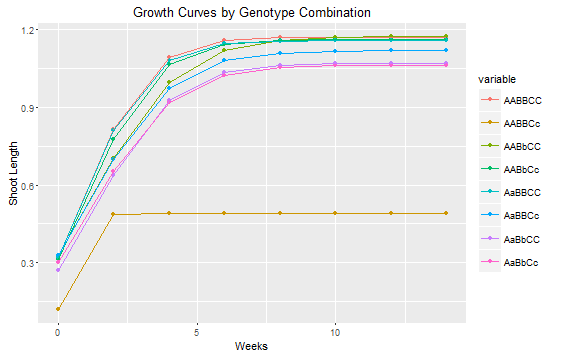
\includegraphics[width=0.8\linewidth]{images/GrowthCurveComparison} 

}

\caption{Growth Curve Comparison}\label{fig:growth-compare}
\end{figure}

\begin{align}
\mu_{111}(t) &= \mu(t) + \alpha_1(t) + \alpha_2(t) + \alpha_3(t) + i_{12}(t) + i_{13}(t) + i_{23}(t) + i_{123}(t)  \notag \\
\mu_{112}(t) &= \mu(t) + \alpha_1(t) + \alpha_2(t) – \alpha_3(t) + i_{12}(t) – i_{13}(t) – i_{23}(t) – i_{123}(t)  \notag \\
\mu_{121}(t) &= \mu(t) + \alpha_1(t) – \alpha_2(t) + \alpha_3(t) – i_{12}(t) + i_{13}(t) – i_{23}(t) – i_{123}(t)  \notag \\
\mu_{122}(t) &= \mu(t) + \alpha_1(t) – \alpha_2(t) – \alpha_3(t) – i_{12}(t) – i_{13}(t) + i_{23}(t) + i_{123}(t)  \notag \\
\mu_{211}(t) &= \mu(t) – \alpha_1(t) + \alpha_2(t) + \alpha_3(t) – i_{12}(t) – i_{13}(t) + i_{23}(t) – i_{123}(t)  \notag \\
\mu_{212}(t) &= \mu(t) – \alpha_1(t) + \alpha_2(t) – \alpha_3(t) – i_{12}(t) + i_{13}(t) – i_{23}(t) + i_{123}(t)  \notag \\
\mu_{221}(t) &= \mu(t) – \alpha_1(t) – \alpha_2(t) + \alpha_3(t) + i_{12}(t) – i_{13}(t) – i_{23}(t) + i_{123}(t)  \notag \\
\mu_{222}(t) &= \mu(t) – \alpha_1(t) – \alpha_2(t) – \alpha_3(t) + i_{12}(t) + i_{13}(t) + i_{23}(t) – i_{123}(t)
\label{eq:genetic-effects}
\end{align}

where \(\mu(t)\) is the population mean at time t; \(\alpha_1(t)\),
\(\alpha_2(t)\), and \(\alpha_3(t)\) are the genetic effects of markers
A, B and C at time t, respectively; \(i_{12}(t)\), \(i_{13}(t)\), and
\(i_{23}(t)\) are the pairwise epistatic effects between markers A and
B, A and C and B and C at time t, respectively; and \(i_{123}(t)\) is
the three-way epistatic effect among three the markers at time t. From
the above equations, we solve the pairwise and three-way epistatic
effects as

\begin{figure}

{\centering 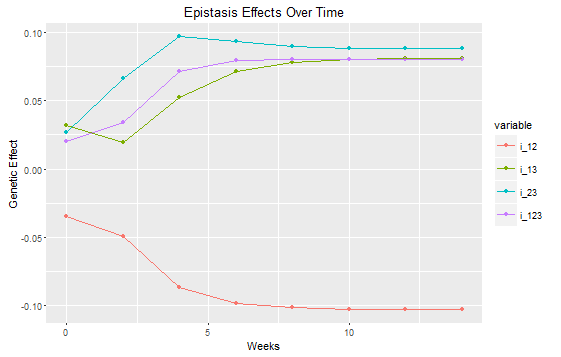
\includegraphics[width=0.8\linewidth]{images/EpistasisComparison} 

}

\caption{Epistasis Comparison}\label{fig:epistasis-compare}
\end{figure}

\begin{align}
i_{12}(t) &=  [(\mu_{111}(t) + \mu_{112}(t) + \mu_{221}(t) + \mu_{222}(t)) – (\mu_{121}(t) + \mu_{122}(t) + \mu_{211}(t) + \mu_{212}(t))] \notag \\
i_{13}(t) &=  [(\mu_{111}(t) + \mu_{121}(t) + \mu_{212}(t) + \mu_{222}(t)) – (\mu_{112}(t) + \mu_{122}(t) + \mu_{211}(t) + \mu_{221}(t))] \notag \\
i_{23}(t) &=  [(\mu_{111}(t) + \mu_{122}(t) + \mu_{211}(t) + \mu_{222}(t)) – (\mu_{112}(t) + \mu_{121}(t) + \mu_{212}(t) + \mu_{221}(t))] \notag \\
i_{123}(t) &=  [(\mu_{111}(t) + \mu_{122}(t) + \mu_{212}(t) + \mu_{122}(t)) – (\mu_{112}(t) + \mu_{121}(t) + \mu_{211}(t) + \mu_{222}(t))]
\label{eq:epi-effects}
\end{align}

Each genotype can draw a growth curve using its growth parameters (a, b,
r) estimated from raw data, from which we can chart the curves of
pairwise and three-way epistatic effects using equation (4). Three
markers AATTC\_nn\_np\_2815, AATTC\_lm\_ll\_3034 and AATTC\_nn\_np\_1615
that produce a significant three-way interaction for parameter x of
shoot length display pronounced differences in growth curve
(\ref{fig:growth-compare}). The epistasis of low- and high-order
performs differently to affect growth form, with three-way interactions
playing a more remarkable role than pairwise epistasis
(\ref{fig:epistasis-compare}).

\section{Discussion}\label{discussion-1}

Genetic interactions have been thought to contribute to a significant
portion of genetic variance for quantitative traits of critical
importance to evolutionary biology, agriculture and medicine (Nelson et
al. 2013; Mackay 2014). While pairwise interactions have been a major
focus of quantitative genetic studies, there has been growing evidence
that genetic interactions involving three or more loci play an important
role in affecting the phenotypic differentiation of traits (Wang et al.
2010; Dowell et al. 2010; Pettersson et al. 2011; Pang et al. 2013;
Weinreich et al. 2013; Taylor and Ehrenreich 2014; Taylor and Ehrenreich
2015). Because of its complexity due to a network of interactions, the
detection of high-order epistasis is extremely difficult (Mackay 2014).
More importantly, interpretation of high-order epistasis and its
contribution to overall genetic architecture can be better made by
jointly analyzing all possible low- and high-order interactions among
genes. This has added an extra challenge to statistical modeling and
detection of this important phenomenon. Thanks to the recent development
of statistical models for high-dimensional variable selection, we have
reformed a statistical modeling framework for detecting high-order
epistasis by focusing on three-way interactions.

Our model extends Hao and Zhang's (2014) forward selection-based
algorithm iFORM that has proven to be robust and efficient for computing
and detecting two-way interactions between predictors (including
continuous predictors). A favorable property of iFORM is its capacity to
detect interactions even if the dimension of predictors is extremely
high relative to a sample size used. The fundamental assumption used by
iFORM is the heredity principle, i.e., the existence of interactions
between a pair of variables that each has at least weak main effects.
After extending it to characterize three-way interactions, this
assumption can be relaxed for the third variable; i.e., even if there is
no detectable main effect for the third marker, then extended iFORM can
still detect the three-way interaction. This property may explain the
reason why high-order epistatic model outperforms low-order epistatic
model, as demonstrated from the detection of significant genetic
interactions in a real data of a woody plant, mei (Prunus mume). It was
found from a recent study that loci participating in high-order genetic
interactions may not individually have measurable effects (Bloom et al.
2013). As a result, our model can be used as a general tool to detect
genetic interactions of various orders and, therefore, elucidate the
overall picture of genetic architecture by capturing the so-called
missing heritability.

The model was investigated by simulation studies whose result help users
to determine an optimal design of mapping or association studies in
terms of sample size, phenotyping precision and the number of markers.
Its application to P. mume genetic mapping leads to the detection of key
loci and their interactions expressed at the low- and high-order levels
for the growth form of shoots. \ldots{}. the R packages was created and
made available through CRAN (Comprehensive R Archive
Network){[}\url{https://cran.r-project.org/}{]}. We packed iFORM/eQTL in
R with the source code is available at Center for Statistical Genetics
(website){[}\url{http://statgen.psu.edu/software/}{]}

\chapter{iForm Functional Mapping (A computational
method)}\label{iform-functional-mapping-a-computational-method}

\section{Motivation}\label{motivation-2}

As we have seen and also has been noted by several researchers while
conducting biometric analysis (\cite{jinks1982biometrical};
\cite{hill2004ds}; \cite{wu1996detecting}) or molecular dissection
(\cite{mackay2009genetics}, \cite{park2010estimation}) is that
quantatitve traits are very complex and much is still needed to be
learned. The researchers cited note that the traits are most likely
polygenic, including gene-gene interactions and other sources of
interaction effects. (\cite{cheverud1995epistasis};
\cite{moore2003ubiquitous}; \cite{van2010detection};
\cite{mackay2014epistasis}) Higher order interactions of complex traits
are not well studied because of their difficulty to detect in mapping
studies as well. The lack of data shoud not be construed as proof that
this order of interaction does not exist. (\cite{taylor2015higher}). The
difficulty in detection leads a way for new computational methods to be
developed and approaches to describe how to distinguish such effects. As
noted in chapter \ref{highorder}, new theoretical models of high-order
epistasis have well been established by mathematical biologists
(\cite{hansen2001epistasis}; \cite{beerenwinkel2007analysis}). These
models provided a foundation to interpret high-order epistasis from a
biological standpoint. A few statistical models have been derived to
estimate and test high-order epistasis in case-control designs
(\cite{wang2015bayesian}) and population-based mapping settings
(\cite{pang2013statistical})

Growth and developmental traits are mostly better described by a
functional process (\cite{hernandez2015understanding},
\cite{muraya2017genetic}), it is more biologically meaningful to map
these traits as growth curves (\cite{sun2015mapping}). There have been a
few different approaches that have integrated growth equations into
genetic mapping via the likelihood function, leading to the birth of a
so-called functional mapping models (\cite{ma2002functional};
\cite{wu2006functional}; \cite{li2015dynamic};
\cite{muraya2017genetic}). These style of appoaches can allow for the
developmental change of genetic control to be characterized across both
time and as well as space (\cite{he2010mapping};
\cite{li2010functional}). Treating the phenotype as a complex trait it
would be likely it would follow a more functional or dynamic process.
This information could be lost or greatly limited by treating the
response as a single static predictor. Modeling the longitudinal
structures in this fashion, functional mapping has proven to be of great
statistical power in gene identification and the utilization of sparse
phenotypic data (\cite{hou2006framework}). In an attempt to capture all
relevant information and be as parsimonuous as possible principles from
biophysical and biochemical processes were considered. The logistic
growth equations are both biologically relevant (\cite{west2001general};
\cite{sun2014model}) and have few parameters that can be mapped to
growth QTLs by estimating these parameters for each genotype and
interactions between genotypes.

There are many approaches for gene mapping with genome-wide association
studies (GWAS) being one of the most popular one, achieving a
considerable success since their first publication in 2005
(\textbackslash{}cite\{klein2005complement). Analytical approaches are
constantly being developed to perform GWAS studies. There are a few
areas of challenges in statistical modeling and analysis of genetic data
that account for the complexity of phenotypic information. Generally
GWAS studies associate genetic markers with static, single valued
phenotypes. As we have discussed, most analysis revolve around pointwise
estimates and do not always take the entirety of the system during the
analysis. Incorporating selecitons are starting to become more common
but further work is this area still needs to be explored. Extending the
forward selecting procedure previously state in \{\#highdeqtl\} and
\{\#highorder\} in order to handle a functional phenotype would be very
beneficial with GWAS level studies. A few challenges do arise while
considering to conduct a genome-wide association study (GWAS) on
interacting traits measured at a sequence of time points. The model
needs to be flexible enough to fit different situations, independence of
the error structure needs to be maintained or accounted for with the
time dependencies and finally computational efficiency needs to be good
enough to fit such complex models. All of these issues combined make it
a difficult exertion to take on but with computational power increasing,
it is becoming more feasible to handle.

In applications like the scenario described where we have a functional
value phenotype and a high dimensional predictor space with dynamically
considering interaciton effects it may be too restrictive to suppose
that the effect of all of the predictors is captured by a simple linear
fit. Reframing the regression problem to help code in the longitudinal
data into the structure of the data in a biologically meaningful manner
and making some sparsity assumptions about the number of significant
genetic and epistatic effects that affect the phenotype will help in the
developement of such a model to tackle such a task.

\section{Methods}\label{methods-2}

\subsection{Regression by linear combination of basis
functions}\label{regression-by-linear-combination-of-basis-functions}

One common approach to regression problems is to frame the model as a
linear combination of basis functions. In typical multiple regression
the design matrix would be the values of the observed predictors and
these would be used to fit the model, usually with a least squares
approach. The goal then being to fit the expected value of the phenotype
of interest in terms of the values of the predictors. This would result
in a linear model of the form,

\begin{equation}
Y = \beta_0 + \beta_1 X_1 + ⋯ + \beta_p X_p + \epsilon
(\#eq: lin-mod)
\end{equation}

This model is nice for a single response but can be too restrictive at
times. With a functional response over time, having a model with more
flexibility could more accurately estimate the phenotype espeically when
considering a functional phenotype like a growth model. A fit like the
one mentioned would only restrict growth to be a straight line and that
may not be applicable in real world applications. By treating the
problem as linear combination of basis functions, the general form would
look like,

\begin{equation}
f(x) = \sum_{i=0}^P \theta_i \phi_i(x)
\label{eq:gen-form}
\end{equation}

where the \(\phi\) are the basis functions of the researchers choosing.
Under this format you can choose any function that would fit the need of
the given problem and has relevance to the application area. A common
choice is to use polynomial regression, where \(/phi\) would be the
predictors raised to different degrees in order to invoke a non-linear
relationship into the model. This works well but it comes with some draw
backs. The first being that for each degree consider, it could grow the
predictor set even larger. Instead of just one effect for each predictor
you could have up to the order of the polynomial effects for each
predictor. With the predictor set being at a high dimensional level
already, this may not be something feasible to do. The other area of
concern is that it would give a way for higher correlation between
effects in the model. This would violate the intial assumptions of the
model.

Standard polynomial regression is just one case of using basis functions
in linear regression. There are many transformations that are able to be
performed to invoke nicer properities to the data. The basis functions
that are going to be focused on in this work are orthogonal polynomials.
This would be a special case of polynomial regression that would
alleviate some of the drawbacks mentioned above. Orthogonal polynomials
by definition are othogonal to each other and therefore would not have
any correlation between predictors when used as basis functions. Also as
an advantage, polynomial regression can be used to make similar types of
interest as other types of multiple regression analysis. It does this
while modeling a non-linear relationship between the phenotype and
genetic markers without having to use complex optimization methods.
Ordinary leasat squares would still apply in this framework, making it
more computational effecient as well. One specific class of othogonal
polynomials that will be used are the Legendre polynomials because of
the nice properites they posses.

\subsection{Legendre Polynomials}\label{legendre-polynomials}

\begin{figure}

{\centering 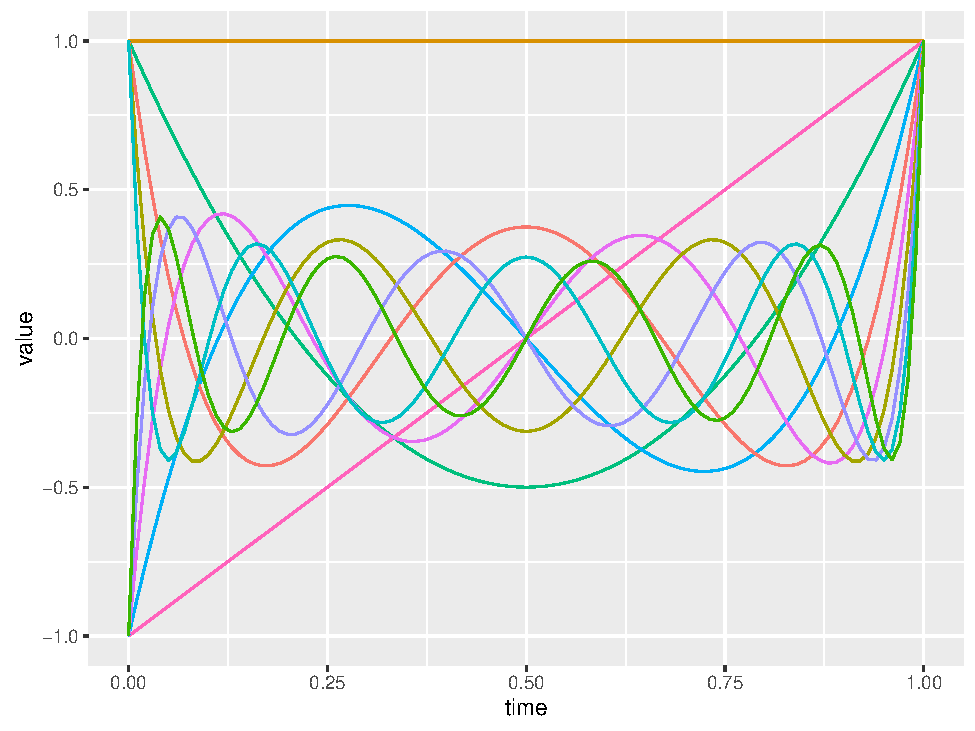
\includegraphics[width=0.8\linewidth]{Defense_files/figure-latex/Legendre-fig-1} 

}

\caption{First 10 Legendre Polynomials}\label{fig:Legendre-fig}
\end{figure}

\textbf{From Wikipedia}

These solutions for n = 0, 1, 2, \ldots{} (with the normalization Pn(1)
= 1) form a polynomial sequence of orthogonal polynomials called the
Legendre polynomials. Each Legendre polynomial Pn(x) is an nth-degree
polynomial. It may be expressed using Rodrigues' formula:

\begin{equation}
P_n(x) = \frac{1}{2^nn!} \frac{d^n}{dx^n}[(x^2-1)^n]
\label{eq:rodrigues-formula}
\end{equation}

An important property of the Legendre polynomials is that they are
orthogonal with respect to the L2-norm on the interval −1 ≤ x ≤ 1:

\begin{equation}
\int_1^{-1} P_m(x)P_n(x)dx = \frac{2}{2+1}\delta_{mn}
\label{eq:orthg-leg}
\end{equation}

\(\delta_{mn}\) denotes teh Kronecker delta equalt to 1 if m = n and 0
otherwise

\begin{equation}
\begin{split}
P_n(x) & = \frac{1}{2^n}\sum_{k=0}^{n}{{n}\choose{k}}^2(x-1)^{n-k}(x+1)^k \\
& = \sum_{k=0}^{n}{{n}\choose{k}}{{-n-1}\choose{k}}{\left(\frac{1-x}{2}\right)}^k \\
& = 2^{-n}\sum_{k=0}^{n} x^k {{n}\choose{k}}{{\frac{n+k+1}{2}}\choose{k}} \\
\end{split}
\label{eq:leg-eq}
\end{equation}

\textbf{free write}

Because the non-parametic nature of the legendre orthogonal polynomials,
it was advantages for both dimension reduction and also handling
unevenly spaced, missing or non-uniform time measurements from different
subjects in the dataset.

The search performed by the procedure checks and uses the legendre
polynomials of different orders to find the best fitting form of the
genetic variation from the mean curve for each of the genotypes or
epistasis between genotypes considered in the model.

\subsection{Model}\label{model}

\textbf{2HIGWAS} Because interaction effects are considered, the
coverage probability P is redefined as three quantities: PA, the
coverage rate of all true predictors; PM, the coverage rate of all main
effects; and PI, the coverage rate of all interaction effects.

\textbf{update} 2HIGWAS \cite{jiang20152higwas}

We consider the complex trait as a growth trait. Thus, it is
biologically meaningful to implement a growth equation, like a logistic
curve, to describe growth trajectory \cite{west2001general}. We describe
the population mean growth curve by the growth equation
\[\mu(t) = a/(1 + b * exp(-r*t))\]

where a, b and r are growth parameters each of biological
interpretation, with a being the asymptotic growth, b being the initial
amount of growth and r being the relative growth rate. Timevarying
additive and dominant effects of significant SNPs are modeled by a
nonparametric approach, such as Legendre orthogonal polynomial used in
quantitative genetic studies
(\cite{olori1999estimating},\cite{li2010functional}{]}, expressed as

\[ \alpha_j(t) = (L_0(t), L_1(t), ... , L_s(t))*(u_{j0}, u_{j1},...,u_{js})^T \]
\[ \beta_j(t) = (L_0(t), L_1(t), ... , L_{s'}(t))*(v_{j0}, v_{j1},...,v_{js'})^T \]

where \(L_0(t), L_1(t), ... , L_s(t)\) and
\(L_0(t), L_1(t), ... , L_{s'}(t)\) are the LOP of orders \(s\) and
\(s'\), respectively; and \(u_{j0}, u_{j1},...,u_{js}\) and
\(v_{j0}, v_{j1},...,v_{js'}\) are the vectors of time-invariant
additive and dominant effects, respectively. Orders \(s\) and \(s'\),
selected from information criteria, such as Akaike information criterion
(AIC) and Bayesian information criterion (BIC), are usually much smaller
than M so that the dimension of response phenotypic data is reduced
through LOP modeling. The variance maxtrix of residual errors is assumed
to follow the first-order structured antedependence {[}SAD(1){]} process
(\cite{li2010functional}). The SAD(1) model has been used in previous
growth modeling studies (\cite{li2010functional},
\cite{ahn2010functional}, \cite{das2011dynamic}).

\textbf{me} The mean growth curve is estimated for the sample and then
orthogonal polynomials are used to assist in fitting the genetic effects
for each marker or epistatic interaction between the markers. This would
allow the genetic effect some flexibility over time and give a more
representative fit. This could also be used with other semi parametric
functions to model dynamics or other types of non-linear functions that
characterizes the biological systems being evaluated.

\textbf{BIC}

Similarly, following the classical BIC rule (Swartz 1978), we can define
the BIC rule for the cubic MESS model as

\[BIC(\lambda, \lambda_v ) = -2*LogLik + log(n)*(df + df_v)\] n is the
number of subjects \cite{wu2006nonparametric}
\[\lambda = smoothing paramter\]
\[\lambda_v = smoothing paramter, number of knots in the cubic spline\]

Considering a comprehensive gentotyping for n progeny each measure
across different time points.

\section{Application}\label{application-2}

\subsection{Simulation Studies}\label{simulation-studies-1}

As statistical issues become more complex they are going to be more
analytically intractable and computational methods will need to close
that gap to show the effectiveness of new models and procedures.

Extensive simulation studies were performed to ascertain the validity of
the model. Computational verified by cross validation, bootstrapping.
Having a training and a testing set to help provide some insight on
false positive rates, selecting the correct fit of the polynomial for
the genetic and epsitatic effects.

\begin{itemize}
\tightlist
\item
  rates at which correct markers/epistasis was selected?
\item
  rates at which the correct order polynomial was fit for the correct
  marker/epistasis
\end{itemize}

\subsection{Worked Example}\label{worked-example-1}

Same mei tree dataset used in previous chapter to see if any new
discoveries can be made by incorporating the time component and fitting
the growth parameters simulatneously throughout the procedure.

if it doesn't take too much time (maybe by the time defense comes
around) cross validate the selection proceudre by leaving out samples
and running model again. How many times do you get the same results?
LOOCV tables

Also consider with holding predictors from the dataset to see if the
selection is changed at all. Start with random ones and then maybe
strategically select important predictors to remove to see how it
affects the fit

\section{Discussion}\label{discussion-2}

\begin{itemize}
\tightlist
\item
  Downfalls or areas of concern for fitting the genetic effects to the
  polynomials?
\item
  How do we know there is epistasis?
\item
  how do you keep it from over selecting
\item
  what if it doesn't follow the heredity or hierarchy principles?
\item
  other types of functional/growth equations to represent biologically
  meaningful scenarios
\end{itemize}

\chapter{Conclusions}\label{conclusions}

** research statement ** Continuing on, my aim would be to work with
datasets of this scale and incorporate the types of statistical methods
mentioned and machine learning techniques to aid in analysis. The
results could help gain larger insights into the genomic/epigenetic
architecture of biological systems. On top of the importance of a
functional component to the phenotype, considering other types of
multivariate responses would be interesting to study in context of such
a system. Integrating different level of omics data and the challenges
that arise with such complicated and large datasets has interested me
throughout my PhD work. Translating such a complex system into usable
information that can be shared in order to prevent and fight disease
would be ideal research for me. This type of research would need both
methodological development as well as application of existing
statistical and machine/deep learning techniques to handle the magnitude
of the problem.

\section{Summary}\label{summary}

applied, adapted and extended the forward selection procedure under the
marginality assumption first proposed by \cite{hao2014interaction}

able to reduce search space substantially by making some reasonable
assumptions about the data. These assumptions can be relaxed a little to
broaden the scope of the space.

advantages

computationally efficient way for high dimensional data situations that
arise from high throughput data, especially when considering epstasis
between gene markers or other type of interaction effects in the model.
Guided search space based off of commonly used principles in model
selection that are relevant in real world situations. Able to perform a
GWAS with included epistatic interactions a fairly quick manner. Able to
relax assumptions to widen the search space. This may decrease the speed
of the algorithm but makes the search more comprehensive. Able to screen
for complex scenarios that would be hard to find in a lab setting
otherwise. Having said that with the flexiblity of the initial model,
false posiive rates could be a concern and need to be taken into
consideration. Adjustement to the significance level and the model
selection criteria have been made to account for this. This would still
need to be followed up on independtly by checking with other datasets
and/or lab verification.

Functional componenets were also considered to such a selection
procedure. This also increases the computational complexity of the model
and therefore decreases some efficeiency gains previously seen. Use
biologically relevant information to guide the fitting of the model.
Initially considers well established growth equations as a baseline for
the underlying structure. It then performs a GWAS level analysis with
considering epstatic interactions throughout the process.

\section{Discussion}\label{discussion-3}

complex and many moving parts to the selection procedure. Very flexible
but this could have it be prone to over fitting at times if not well
controlled. Need to heavily consider this as part of interpretating the
model. Mainly used a screening to guide future research.

With the complexity and expense that comes with genetic mapping,
espically with a functional trait that needs repeated measuresUsed as a
screening tool for initial findings and exploratory data analysis to aid
and guide future research. Needs to be then be lab validated. Especially
with something as intricate as epistatic effects between gene markers.

Further investigations are needed to confirm or modify our findings by
QTL mapping in natural populations.

\textbf{BIC Limitations (wikipedia)} the above approximation is only
valid for sample size n much larger than the number k of parameters in
the model.

the BIC cannot handle complex collections of models as in the variable
selection (or feature selection) problem in high-dimension.{[}3{]}

\section{Future Steps}\label{future-steps}

\subsection{Aim 1}\label{aim-1}

incorporate other mean curves for intercept term Other types of
orthogonal polynomials general additive models components

consider different level of interactions and omics data.
gene-environment methylation

\subsection{Aim 2}\label{aim-2}

extend to include multivariate reponses to the system how to extend
selection criteria in this fashion search space grows even larger what
is defined as the `best' predictor for 1 reponse might not be for the
others

\subsection{Aim 3}\label{aim-3}

We have finished a nice book.

\chapter{Appendix}\label{appendix}

This needs more work. Only includes first part of the appendix pdf

\begin{center} 
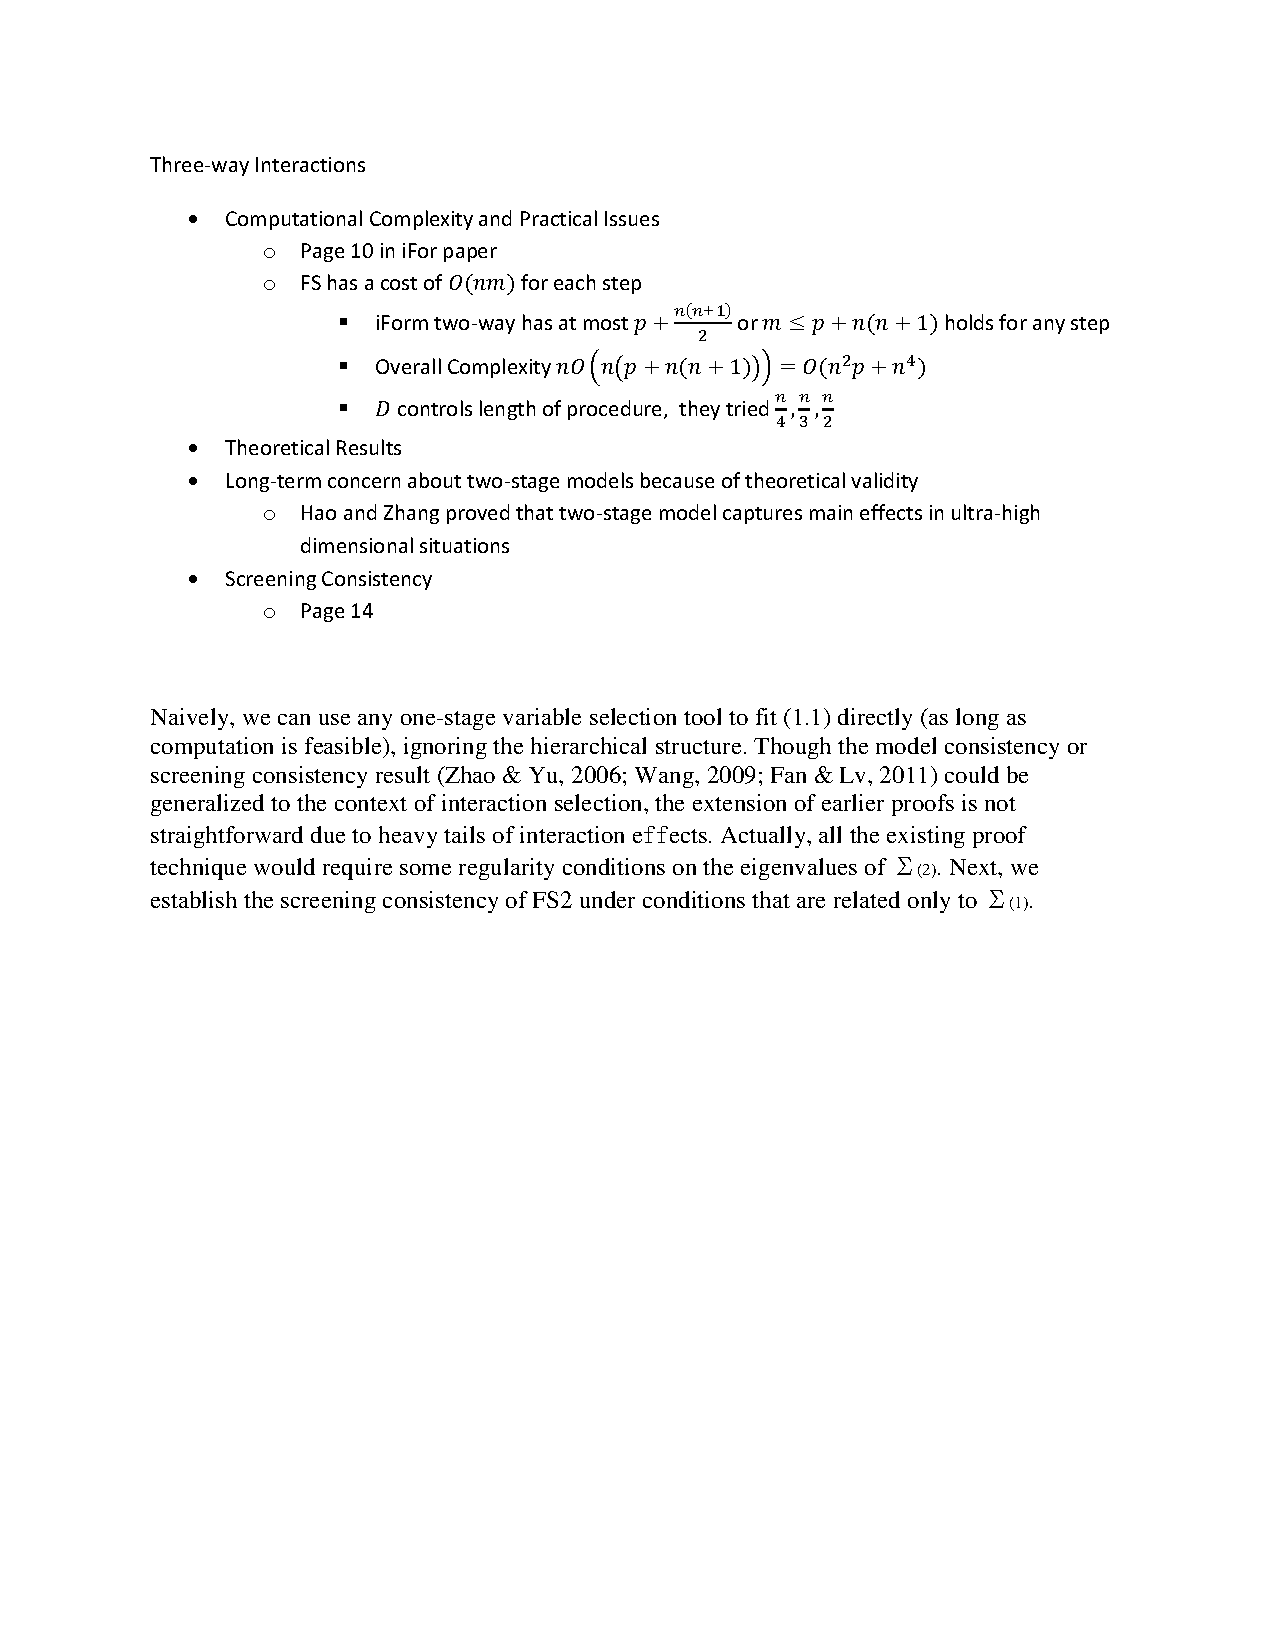
\includegraphics[width=8in]{appendix.pdf} 
\end{center}

\bibliography{packages,book}
\addcontentsline{toc}{chapter}{\bibname}


\end{document}
